% =====================================================================
% Capítulo 2 — Sequências e Séries
% Seção 2.1 (tradução para PT-BR de Abbott, Understanding Analysis,
% 2ª ed., páginas 50–52 do OCR). O título do capítulo deve ser
% declarado no arquivo principal.
% =====================================================================

\index[remissivo]{série!infinita} \index[remissivo]{rearranjo}
\section{Discussão: Reordenamentos de Séries Infinitas}\label{sec2:reordenamentos-series}

O Capítulo~2 trata de sequências e séries infinitas, enfatizando como operações aparentemente familiares devem ser interpretadas quando envolvem infinitos termos.

Considere a série infinita
\[
\sum_{n=1}^{\infty} \frac{(-1)^{n+1}}{n} \index[remissivo]{série!harmônica} \index[remissivo]{série!harmônica!alternada}
 = 1 - \frac{1}{2} + \frac{1}{3} - \frac{1}{4} + \frac{1}{5} - \frac{1}{6} + \frac{1}{7} - \frac{1}{8} + \cdots.
\]
Se começarmos ingenuamente a somar da esquerda para a direita, obteremos uma sequência das chamadas \textit{somas parciais}. Em outras palavras, seja $s_n$ a soma dos primeiros $n$ termos da série; assim, $s_1=1$, $s_2=1/2$, $s_3=5/6$, $s_4=7/12$, e assim por diante. Uma observação imediata é que as somas sucessivas oscilam dentro de um intervalo progressivamente menor. As somas ímpares decrescem ($s_1>s_3>s_5>\dots$), enquanto as somas pares crescem ($s_2<s_4<s_6<\dots$). \index[remissivo]{soma!parcial}

% Ordem das somas parciais pares e ímpares.
\begin{center}
\begin{tikzpicture}[x=13.5cm,y=1cm]
  % Intervalo de referência.
  \draw[thick, -stealth] (0,0) -- (1.12,0);
  \draw (0,-0.08) -- (0,0.08) node[below=5pt] {$0$};
  \draw (1,-0.01) -- (1,0.01) node[below=5pt] {$1$};

  % Somas parciais e limite aproximado.
  \fill (0.5,0) circle (1.8pt) node[above=3pt] {$s_2$};
  \fill (0.5833,0) circle (1.8pt)
    node[above=3pt,xshift=-2pt] {$s_4$};
  \fill (0.6167,0) circle (1.8pt)
    node[above=3pt,xshift=4pt] {$s_6$};
  \fill (0.69,0) circle (1.8pt);
  \draw[thick, -stealth] (0.69,0.95) -- (0.69,0.2)
    node[pos=0,above] {$S\mathrel{\approx}0{,}69$};
  \fill (0.7833,0) circle (1.8pt) node[above=3pt] {$s_5$};
  \fill (0.8333,0) circle (1.8pt) node[above=3pt] {$s_3$};
  \fill (1,0) circle (1.8pt) node[above=3pt] {$s_1$};
\end{tikzpicture}
\end{center}

\[
s_2 < s_4 < s_6 < \cdots < s_5 < s_3 < s_1
\]

Parece razoável --- e em breve provaremos isso --- que a sequência $(s_n)$ se aproxime cada vez mais de um valor, digamos $S$, no qual as somas parciais ímpares e pares ``se encontram''. Neste momento, não podemos calcular $S$ com precisão, mas sabemos que ele está entre $7/12$ e $5/6$. Somar algumas centenas de termos revela que $S\approx 0{,}69$. Qualquer que seja seu valor, surge então uma tentação irresistível de escrever \index[remissivo]{sequência}
\[
\tag{1}
S=1-\frac{1}{2}+\frac{1}{3}-\frac{1}{4}+\frac{1}{5}-\frac{1}{6}+\frac{1}{7}-\frac{1}{8}+\cdots,
\]
querendo dizer, talvez, que, se pudéssemos de fato somar todos esses números infinitamente numerosos, então a soma seria igual a $S$. Um exemplo mais familiar de uma equação desse tipo é
\[
2=1+\frac{1}{2}+\frac{1}{4}+\frac{1}{8}+\frac{1}{16}+\frac{1}{32}+\frac{1}{64}+\cdots,
\]
a única diferença sendo que, na segunda equação, temos um valor mais reconhecível para a soma.

Mas agora chegamos ao ponto crucial. Os símbolos $+$, $-$ e $=$ nas equações anteriores são noções enganosamente familiares, empregadas de uma maneira muito pouco familiar. A questão decisiva é saber se as propriedades da adição e da igualdade, bem compreendidas para somas finitas, continuam válidas quando aplicadas a objetos infinitos como a equação (1). A resposta, como veremos, é um tanto ambígua.

Tratando a equação (1) de maneira algébrica usual e multiplicando ambos
lados por $1/2$ e em seguida, somando o resultado obtido à própria equação (1), ficamos com o 
resultado que aparece na terceira linha abaixo:
\begin{align}
 \frac{1}{2}S &= \frac{1}{2}-\frac{1}{4}+\frac{1}{6}-\frac{1}{8}+\frac{1}{10}-\frac{1}{12}+\cdots 
 \nonumber\\[0.1cm]
 &+
 \nonumber\\[0.1cm]
 S\phantom{0} &= 1-\frac{1}{2}+\frac{1}{3}-\frac{1}{4}+\frac{1}{5}-
 \frac{1}{6}+\frac{1}{7}-\frac{1}{8}+\frac{1}{9}-\frac{1}{10}
 +\frac{1}{11}-\frac{1}{12}+\frac{1}{13}-\cdots 
\nonumber\\[0.6cm]
{}
\frac{3}{2}S &= 1+\frac{1}{3}-\frac{1}{2}+\frac{1}{5}+\frac{1}{7}-\frac{1}{4}+\frac{1}{9}+\frac{1}{11}-\frac{1}{6}+\frac{1}{13}+\cdots
\tag{2}
\end{align}

Agora, observe atentamente o resultado. A soma na equação (2) consiste precisamente dos mesmos termos da equação original (1), apenas em uma ordem diferente. Mais especificamente, a série em (2) é um reordenamento de (1) no qual listamos os dois primeiros termos positivos $(1+1/3)$, seguidos pelo primeiro termo negativo $(-1/2)$; depois, os dois termos positivos seguintes $(1/5+1/7)$, seguidos pelo termo negativo seguinte $(-1/4)$. Continuando dessa maneira, fica claro que todo termo de (2) aparece em (1), e vice-versa. O problema surge quando percebemos que a equação (2) afirma que a soma desses números reordenados, embora inalterados, é igual a $3/2$ do valor original. De fato, a soma de algumas centenas de termos da equação (2) produz somas parciais próximas de $1{,}03$. Nesse contexto infinito, a adição não é comutativa! \index[remissivo]{rearranjo}

Vejamos um reordenamento semelhante da série
\[
\sum_{n=0}^{\infty}(-1/2)^n.
\]
Essa série é geométrica, com primeiro termo igual a $1$ e razão comum $r=-1/2$. Usando a fórmula $1/(1-r)$ para a soma de uma série geométrica (\Cref{exmpl:2-7-5}), obtemos \index[remissivo]{série!geométrica} \index[remissivo]{série!geométrica!razão}
\[
1-\frac{1}{2}+\frac{1}{4}-\frac{1}{8}+\frac{1}{16}-\frac{1}{32}+\frac{1}{64}-\frac{1}{128}+\frac{1}{256}+\cdots
=\frac{1}{1-(-\frac{1}{2})}=\frac{2}{3}.
\]
Desta vez, alguma experimentação computacional com o reordenamento ``dois positivos, um negativo'',
\[
1+\frac{1}{4}-\frac{1}{2}+\frac{1}{16}+\frac{1}{64}-\frac{1}{8}+\frac{1}{256}+\frac{1}{1024}-\frac{1}{32}+\cdots,
\]
produz somas parciais bastante próximas de $2/3$. A soma dos primeiros $30$ termos, por exemplo, é igual a $0{,}666667$. A adição infinita é comutativa em alguns casos, mas não em outros.

Longe de ser uma encantadora curiosidade teórica das séries infinitas, esse fenômeno pode ser fonte de grande consternação em muitas situações aplicadas. Como, por exemplo, deveria ser definida uma soma dupla sobre duas variáveis de índice? Suponhamos que nos seja dada uma grade de números reais $\{a_{ij}:i,j\in\mathbb{N}\}$, em que \index[remissivo]{soma!dupla}
\[
a_{ij}=\begin{cases}
1/2^{j-i},& j>i,\\
-1,& j=i,\\
0,& j<i.
\end{cases}
\]
Essa grade é
\[
\renewcommand{\arraystretch}{2.2}
\setlength{\arraycolsep}{10pt}
\begin{bmatrix}
-1&\dfrac12&\dfrac14&\dfrac18&\dfrac1{16}&\cdots\\
0&-1&\dfrac12&\dfrac14&\dfrac18&\cdots\\
0&0&-1&\dfrac12&\dfrac14&\cdots\\
0&0&0&-1&\dfrac12&\cdots\\
0&0&0&0&-1&\cdots\\
\vdots&\vdots&\vdots&\vdots&\vdots&\ddots
\end{bmatrix}.
\]

Gostaríamos de atribuir um significado matemático à soma
\[
\sum_{i,j=1}^{\infty}a_{ij},
\]
pretendendo incluir no total todos os termos da matriz anterior. Uma ideia natural é fixar temporariamente $i$ e somar ao longo de cada linha. Um instante de reflexão (e um fato sobre séries geométricas) mostra que cada linha tem soma igual a $0$. Somando as somas das linhas, obtemos \index[remissivo]{soma!dupla!iterada}
\[
\sum_{i,j=1}^{\infty}a_{ij}
=\sum_{i=1}^{\infty}\left(\sum_{j=1}^{\infty}a_{ij}\right)
=\sum_{i=1}^{\infty}(0)=0.
\]

Poderíamos igualmente ter decidido fixar $j$ e somar primeiro ao longo de cada coluna. Nesse caso,
\[
\sum_{i,j=1}^{\infty}a_{ij}
=\sum_{j=1}^{\infty}\left(\sum_{i=1}^{\infty}a_{ij}\right)
=\sum_{j=1}^{\infty}\left(\frac{-1}{2^{j-1}}\right)=-2.
\]

Mudar a ordem da soma muda o valor da soma! Uma maneira comum de surgirem somas duplas (embora não esta em particular) é por meio do produto de duas séries. Há uma tendência natural a escrever \index[remissivo]{produto!de Cauchy}
\[
\left(\sum a_i\right)\left(\sum b_j\right)=\sum_{i,j}a_i b_j,
\]
mas, no momento, a expressão do lado direito não faz sentido.

São essas patologias que dão origem à necessidade de rigor. Uma resolução satisfatória das questões levantadas exigirá que sejamos absolutamente precisos quanto ao que queremos dizer ao manipular esses objetos infinitos. No início, o progresso pode parecer lento, mas isso se deve ao fato de não querermos cair na armadilha de deixar que os vieses de nossa intuição corrompam nossos argumentos. Demonstrações rigorosas destinam-se a servir de freio à intuição e, ao final, veremos que elas melhoram imensamente nossa imagem mental do infinito matemático.

Como exemplo final, considere algo tão intuitivamente fundamental quanto a propriedade associativa da adição aplicada à série $\sum_{n=1}^{\infty}(-1)^{n}$. Agrupando os termos de uma maneira, obtemos
\[
(-1 + 1) + (-1 + 1) + (-1 + 1) + (-1 + 1) + \cdots = 0 + 0 + 0 + 0 + \cdots = 0,
\]
ao passo que, agrupando-os de outra,
\[
-1 + (1 - 1) + (1 - 1) + (1 - 1) + \cdots = -1 + 0 + 0 + 0 + \cdots = -1.
\]
Manipulações legítimas em contextos finitos nem sempre se estendem a contextos infinitos. Decidir quando elas valem e por que não valem é um dos temas centrais da análise.

% ---------------------------------------------------------------------
% Seção 2.2 — O Limite de uma sequência
% (tradução para PT-BR de Abbott, Understanding Analysis, 2ª ed.,
% páginas 53–59 do OCR).
% ---------------------------------------------------------------------
% NOTA: o trecho inicial da página 53 do OCR ("It is the pathologies..."
% e o exemplo da associatividade em sum (-1)^n) pertence à Seção 2.1
% (Discussão) e não foi incluído aqui.

\index[remissivo]{limite de sequência}
\section{O Limite de uma sequência}\label{sec2:limite-sequencia}

A compreensão de séries infinitas depende fortemente de uma compreensão clara da teoria das sequências. De fato, a maioria dos conceitos da análise pode ser reduzida a afirmações sobre o comportamento de sequências. Assim, dedicaremos um tempo significativo ao estudo das sequências antes de enfrentar as séries infinitas.

\begin{definition}\label{def:sequencia}
Uma \textit{sequência} é uma função cujo domínio é $\mathbb{N}$. \index[remissivo]{sequência} \index[remissivo]{função} \index[remissivo]{função!domínio}
\end{definition}

Essa definição formal leva imediatamente à representação familiar de uma sequência como uma lista ordenada de números reais. Dada uma função $f \colon \mathbb{N} \to \mathbb{R}$, $f(n)$ é simplesmente o $n$-ésimo termo da lista. A notação para sequências reforça essa compreensão familiar.

\begin{example}\label{exmpl:2-2-2}
Cada uma das formas a seguir é uma maneira comum de descrever uma sequência.
\begin{enumerate}[label=(\roman*)]
\item $\left(1, \frac{1}{2}, \frac{1}{3}, \frac{1}{4}, \cdots\right)$,
\item $\left(\frac{1+n}{n}\right)_{n=1}^{\infty} = \left(\frac{2}{1}, \frac{3}{2}, \frac{4}{3}, \cdots\right)$,
\item $(a_n)$, onde $a_n = 2^n$ para cada $n \in \mathbb{N}$,
\item $(x_n)$, onde $x_1 = 2$ e $x_{n+1} = \frac{x_n+1}{2}$.
\end{enumerate}
\end{example}

Em certas ocasiões, será mais conveniente indexar uma sequência começando com $n = 0$ ou $n = n_0$, para algum número natural $n_0$ diferente de $1$. Essas pequenas variações não devem causar confusão. O que é essencial é que uma sequência seja uma lista \textit{infinita} de números reais. O que acontece no início de tal lista é de pouca importância na maioria dos casos. O que interessa à análise é o comportamento da ``cauda'' infinita de uma dada sequência. \index[remissivo]{sequência!cauda}

Apresentamos agora aquela que é, possivelmente, a definição mais importante deste livro.

\begin{definition}[Convergência de uma sequência]\label{def:convergencia-sequencia}
Uma sequência $(a_n)$ \textit{converge} para um número real $a$ se, para todo número positivo $\epsilon$, existe $N \in \mathbb{N}$ tal que, sempre que $n \geq N$, segue que $|a_n - a| < \epsilon$. \index[remissivo]{convergência} \index[remissivo]{limite de sequência} \index[remissivo]{limite de sequência!definição epsilon-N@definição \(\varepsilon\)--\(N\)}
\end{definition}

Para indicar que $(a_n)$ converge para $a$, costumamos escrever $\lim a_n = a$ ou $(a_n) \to a$. A notação $\lim_{n \to \infty} a_n = a$ também é padrão.

Num esforço para decifrar essa definição complicada, ajuda considerar primeiro a frase final ``$|a_n - a| < \epsilon$'' e pensar sobre os pontos que satisfazem uma desigualdade desse tipo.

\begin{definition}[$\epsilon$-vizinhança]\label{def:vizinhanca-epsilon}
Dado um número real $a \in \mathbb{R}$ e um número positivo $\epsilon > 0$, o conjunto
\[
V_\epsilon(a) = \{x \in \mathbb{R} : |x - a| < \epsilon\}
\]
é chamado de \textit{$\epsilon$-vizinhança} de $a$. \index[remissivo]{epsilon-vizinhança@\(\varepsilon\)-vizinhança}
\end{definition}

Observe que $V_\epsilon(a)$ consiste em todos os pontos cuja distância a $a$ é menor que $\epsilon$. Dito de outra forma, $V_\epsilon(a)$ é um intervalo, centrado em $a$, com raio $\epsilon$.

% A $\epsilon$-vizinhança $V_\epsilon(a)$ como intervalo centrado em $a$.
\begin{center}
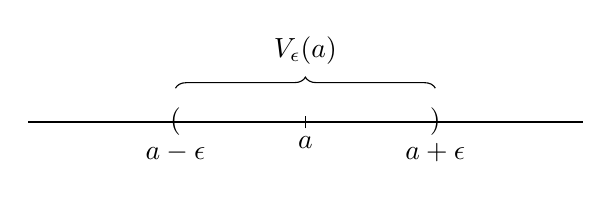
\begin{tikzpicture}[x=2.2cm,y=1cm]
  % Reta real, com o intervalo aberto destacado entre a-epsilon e a+epsilon.
  \draw (-1.6,0) -- (1.6,0);
  \node[anchor=center, inner sep=0pt] at (-0.75,0) {$($};
  \node[anchor=center, inner sep=0pt] at (0.75,0) {$)$};

  % Pontos de referência e respectivas coordenadas.
  \draw (0,-0.08) -- (0,0.08)
    node[below=4pt] {$a$};
  \node[below=4pt] at (-0.75,0) {$a-\epsilon$};
  \node[below=4pt] at (0.75,0) {$a+\epsilon$};

  % Chave superior para identificar a vizinhanca.
  \draw[decorate, decoration={brace, amplitude=4pt}]
    (-0.75,0.43) -- (0.75,0.43)
    node[midway, above=5pt] {$V_\epsilon(a)$};
\end{tikzpicture}
\end{center}

Reformular a definição de convergência em termos de $\epsilon$-vizinhanças dá uma impressão mais geométrica do que está sendo descrito.

\begin{definition}[Convergência de uma sequência: Versão Topológica]\label{def:convergencia-topologica}
Uma sequência $(a_n)$ converge para $a$ se, dada qualquer $\epsilon$-vizinhança $V_\epsilon(a)$ de $a$, existe um ponto da sequência a partir do qual todos os termos estão em $V_\epsilon(a)$. Em outras palavras, toda $\epsilon$-vizinhança contém todos os termos de $(a_n)$, exceto um número finito deles. \index[remissivo]{convergência}
\end{definition}

% Interpretação topológica da convergência: todos os termos, exceto um
% número finito, dentro de $V_\epsilon(a)$.
\begin{center}
\begin{tikzpicture}[x=4.2cm,y=1cm]
  % Reta real, com seta stealth apenas no lado direito.
  \draw[-stealth] (-1.6,0) -- (1.85,0);

  % A vizinhança aberta, com os parêntesis centrados na reta.
  \node[anchor=center, inner sep=0pt] at (0.15,0) {$($};
  \node[anchor=center, inner sep=0pt] at (1.15,0) {$)$};
  \node[below=4pt] at (0.15,0) {$a-\epsilon$};
  \node[below=4pt] at (0.65,0) {$a$};
  \node[below=4pt] at (1.15,0) {$a+\epsilon$};
  \draw[line width=0.8pt] (0.65,-0.10) -- (0.65,0.10);

  % Chave superior para V_epsilon(a).
  \draw[decorate, decoration={brace, amplitude=4pt}]
    (0.15,1) -- (1.15,1)
    node[midway, above=5pt] {$V_\epsilon(a)$};

  % Os primeiros termos podem estar fora da vizinhança.
  \foreach \x in {-1.02,-0.68,-0.34,-0.05} {
    \fill (\x,0) circle (2pt);
  }
  \node[above=5pt] at (-1.02,0) {$a_1$};
  \node[above=5pt] at (-0.68,0) {$a_2$};
  \node[above=5pt] at (-0.34,0) {$a_3$};
  \node[above=4pt] at (-0.18,0) {$\cdots$};

  % A partir de a_N, os termos permanecem na epsilon-vizinhança.
  \fill (0.28,0) circle (2pt);
  \node[above=5pt] at (0.28,0.35) {$a_N$};
  \draw[thick,-stealth] (0.28,0.55) -- (0.28,0.15);
  \foreach \x in {0.40,0.50,0.58,0.62,0.66,0.70,0.74,0.78,0.86,0.96,1.08} {
    \fill (\x,0) circle (2pt);
  }
\end{tikzpicture}
\end{center}

A \Cref{def:convergencia-sequencia} e a \Cref{def:convergencia-topologica} dizem precisamente a mesma coisa; o número natural $N$ na versão original da definição é o ponto em que a sequência $(a_n)$ entra em $V_\epsilon(a)$, para nunca mais sair. Deve ficar claro que \textit{o valor de $N$ depende da escolha de $\epsilon$}. Quanto menor a $\epsilon$-vizinhança, maior pode ter que ser $N$.

\begin{example}\label{exmpl:2-2-5}
Considere a sequência $(a_n)$, onde $a_n = 1/\sqrt{n}$.

Nossa compreensão intuitiva de limites aponta com segurança para a conclusão de que
\[
\lim \left( \frac{1}{\sqrt{n}} \right) = 0.
\]
Antes de tentar provar esse fato não muito impressionante, vamos primeiro explorar a relação entre $\epsilon$ e $N$ na definição de convergência. Por enquanto, tome $\epsilon = 1/10$. Isso define uma espécie de ``zona-alvo'' para os termos da sequência. Ao afirmar que o limite de $(a_n)$ é $0$, estamos dizendo que os termos desta sequência ficam, eventualmente, arbitrariamente próximos de $0$. Quão próximos? O que queremos dizer com ``eventualmente''? Estabelecemos $\epsilon = 1/10$ como nosso padrão de proximidade, o que leva à $\epsilon$-vizinhança $(-1/10, 1/10)$ centrada no limite $0$. Até onde devemos avançar na sequência antes que os termos caiam nesse intervalo? O centésimo termo $a_{100} = 1/10$ nos coloca exatamente sobre a fronteira, e uma pequena reflexão revela que
\[
\text{se} \quad n > 100, \quad \text{então} \quad a_n \in \left( -\frac{1}{10}, \frac{1}{10} \right).
\]
Assim, para $\epsilon = 1/10$, escolhemos $N = 101$ (ou qualquer valor maior) como nossa resposta.

Nossa escolha de $\epsilon = 1/10$ foi bastante arbitrária, e podemos repetir o processo, tomando $\epsilon = 1/50$. Nesse caso, nossa vizinhança-alvo encolhe para $(-1/50, 1/50)$, e fica claro que devemos avançar mais na sequência antes que $a_n$ caia nesse intervalo. Até onde? Essencialmente, precisamos que
\[
\frac{1}{\sqrt{n}} < \frac{1}{50} \quad \text{o que ocorre desde que} \quad n > 50^2 = 2500.
\]
Assim, $N = 2501$ é uma resposta adequada ao desafio de $\epsilon = 1/50$.

Pode parecer que esse duelo poderia continuar para sempre, com diferentes desafios $\epsilon$ sendo lançados um após outro, cada um exigindo um valor adequado de $N$ como resposta. Em certo sentido, isso está correto, exceto pelo fato de que o jogo está efetivamente terminado no instante em que reconhecemos uma regra para escolher $N$ dado um $\epsilon > 0$ arbitrário. Para este problema, o algoritmo desejado está implícito na álgebra feita para calcular a resposta anterior $N = 2501$. Qualquer que seja $\epsilon$, queremos
\[
\frac{1}{\sqrt{n}} < \epsilon \quad \text{o que é equivalente a insistir que} \quad n > \frac{1}{\epsilon^2}.
\]
Com essa observação, estamos prontos para escrever o argumento formal.

Afirmamos que
\[
\lim \left( \frac{1}{\sqrt{n}} \right) = 0.
\]

\begin{proof}
Seja $\epsilon > 0$ um número positivo arbitrário. Escolha um número natural $N$ satisfazendo
\[
N > \frac{1}{\epsilon^2}.
\]
Verificamos agora que essa escolha de $N$ tem a propriedade desejada. Seja $n \geq N$. Então,
\[
n > \frac{1}{\epsilon^2} \quad \text{implica} \quad \frac{1}{\sqrt{n}} < \epsilon, \quad \text{e portanto} \quad |a_n - 0| < \epsilon. \qedhere
\]
\end{proof}
\end{example}

\index[remissivo]{quantificador}
\subsection{Quantificadores}

A definição de convergência dada anteriormente é o resultado de centenas de anos de refinamento da noção intuitiva de limite em um enunciado matematicamente rigoroso. A lógica envolvida é complicada e está intimamente ligada ao uso dos quantificadores ``para todo'' e ``existe''. Aprender a escrever uma prova de convergência gramaticalmente correta anda de mãos dadas com uma compreensão profunda de por que os quantificadores aparecem na ordem em que aparecem.

A definição começa com a frase
\[
\text{``Para todo } \epsilon > 0, \text{ existe } N \in \mathbb{N} \text{ tal que } \dots\text{''}
\]
Olhando para o nosso primeiro exemplo, vemos que nossa prova formal começa com ``Seja $\epsilon > 0$ um número positivo arbitrário.'' Em seguida, vem uma construção de $N$ e, depois, uma demonstração de que essa escolha de $N$ tem a propriedade desejada. Esse é, de fato, um esboço básico de como toda prova de convergência deve ser apresentada.

\textbf{Modelo para uma prova de que $(x_n) \to x$:}
\begin{itemize}
\item ``Seja $\epsilon > 0$ arbitrário.''
\item Apresente uma escolha para $N \in \mathbb{N}$. Essa etapa geralmente é a que exige mais trabalho, quase todo ele feito antes de se escrever a prova formal propriamente dita.
\item Agora, mostre que esse $N$ de fato funciona.
  \begin{itemize}
  \item ``Suponha $n \geq N$.''
  \item Com $N$ bem escolhido, deve ser possível derivar a desigualdade $|x_n - x| < \epsilon$.
  \end{itemize}
\end{itemize}

\begin{example}\label{exmpl:2-2-6}
Mostre que
\[
\lim \left( \frac{n+1}{n} \right) = 1.
\]

Como mencionado, antes de tentar uma prova formal, precisamos primeiro fazer algum rascunho preliminar. No primeiro exemplo, experimentamos atribuir valores específicos a $\epsilon$ (e não é má ideia fazer isso de novo), mas vamos pular direto para a conclusão algébrica. A última linha de nossa prova deve ser que, para valores suficientemente grandes de $n$,
\[
\left| \frac{n+1}{n} - 1 \right| < \epsilon.
\]
Como
\[
\left| \frac{n+1}{n} - 1 \right| = \frac{1}{n},
\]
isso é equivalente à desigualdade $1/n < \epsilon$, ou $n > 1/\epsilon$. Assim, escolher $N$ como um inteiro maior que $1/\epsilon$ será suficiente.

Com o trabalho da prova concluído, tudo o que resta é a redação formal.

\begin{proof}
Seja $\epsilon > 0$ arbitrário. Escolha $N \in \mathbb{N}$ com $N > 1/\epsilon$. Para verificar que essa escolha de $N$ é apropriada, seja $n \in \mathbb{N}$ satisfazendo $n \geq N$. Então, $n \geq N$ implica $n > 1/\epsilon$, que é o mesmo que dizer $1/n < \epsilon$. Finalmente, isso significa
\[
\left| \frac{n+1}{n} - 1 \right| < \epsilon,
\]
como desejado.
\end{proof}
\end{example}

É instrutivo ver o que dá errado no exemplo anterior se tentarmos provar que nossa sequência converge para algum limite diferente de $1$.

\begin{theorem}[Unicidade do Limite]\label{thm:unicidade-limite}
O limite de uma sequência, quando existe, deve ser único.
\end{theorem}

\begin{proof}
\Cref{ex:2-2-6}.
\end{proof}

\subsection{Divergência}

Uma compreensão significativa do papel dos quantificadores na definição de convergência pode ser obtida estudando um exemplo de sequência que não possui limite.

\begin{example}\label{exmpl:2-2-8}
Considere a sequência
\[
\left( 1, -\frac{1}{2}, \frac{1}{3}, -\frac{1}{4}, \frac{1}{5}, -\frac{1}{5}, \frac{1}{5}, -\frac{1}{5}, \frac{1}{5}, -\frac{1}{5}, \frac{1}{5}, -\frac{1}{5}, \frac{1}{5}, -\frac{1}{5}, \dots \right).
\]
Como podemos argumentar que essa sequência não converge para zero? Olhando os primeiros termos, parece que a evidência inicial de fato apoia tal conclusão. Dado um desafio de $\epsilon = 1/2$, uma pequena reflexão revela que, após $N = 3$, todos os termos caem na vizinhança $(-1/2, 1/2)$. Também poderíamos lidar com $\epsilon = 1/4$. (Qual é o menor $N$ possível nesse caso?)

Mas a definição de convergência diz ``\textit{Para todo $\epsilon > 0 \dots$}'', e deve ficar claro que não há resposta para uma escolha de $\epsilon = 1/10$, por exemplo. Isso nos leva a uma observação importante sobre a negação lógica da definição de convergência de uma sequência. Para provar que um determinado número $x$ \textit{não} é o limite de uma sequência $(x_n)$, devemos produzir um único valor de $\epsilon$ para o qual nenhum $N \in \mathbb{N}$ funciona. De modo mais geral, a negação de um enunciado que começa com ``Para todo P, existe Q\dots'' é o enunciado ``Para pelo menos um P, nenhum Q é possível\dots''. Por exemplo, como poderíamos refutar a afirmação falsa de que ``Em toda universidade dos Estados Unidos, existe um aluno com pelo menos sete pés de altura''?

Argumentamos que a sequência anterior não converge para $0$. Vamos agora argumentar contra a afirmação de que ela converge para $1/5$. Escolher $\epsilon = 1/10$ produz a vizinhança $(1/10, 3/10)$. Embora a sequência revisite continuamente essa vizinhança, não há um ponto a partir do qual ela entre e nunca mais saia, como a definição exige. Assim, não existe $N$ para $\epsilon = 1/10$, de modo que a sequência não converge para $1/5$.
\end{example}

É claro que essa sequência não converge para nenhum outro número real, e seria mais satisfatório dizer simplesmente que essa sequência não converge.

\begin{definition}\label{def:divergencia}
Uma sequência que não converge é dita \textit{divergente}. \index[remissivo]{divergência}
\end{definition}

Embora não seja muito difícil, adiaremos a argumentação sobre divergência em geral até desenvolvermos um critério de divergência mais econômico, mais adiante, na \Cref{sec2:subsequencias-bolzano-weierstrass}.

\subsection{Lista de Exercícios}\label{subsec:exercicios-limite-sequencia}

\begin{exercise}\label{ex:2-2-1}
O que acontece se invertermos a ordem dos quantificadores na \Cref{def:convergencia-sequencia}?

\noindent\textit{Definição:} Uma sequência $(x_n)$ \textit{ver-con-ge} para $x$ se \textit{existe} $\epsilon > 0$ tal que, \textit{para todo} $N \in \mathbb{N}$, é verdade que $n \geq N$ implica $|x_n - x| < \epsilon$.

Dê um exemplo de uma sequência ver-con-gente. Existe um exemplo de uma sequência ver-con-gente que seja divergente? Pode uma sequência ver-con-gir para dois valores diferentes? O que exatamente está sendo descrito nessa estranha definição?
\end{exercise}

\begin{exercise}\label{ex:2-2-2}
Verifique, usando a definição de convergência de uma sequência, que as seguintes sequências convergem para o limite proposto.
\begin{enumerate}[label=\alph*)]
\item $\displaystyle\lim_{n\to\infty} \frac{2n+1}{5n+4} = \frac{2}{5}$.
\item $\displaystyle\lim_{n\to\infty} \frac{2n^2}{n^3+3} = 0$.
\item $\displaystyle\lim_{n\to\infty} \frac{\sin(n^2)}{\sqrt[3]{n}} = 0$.
\end{enumerate}
\end{exercise}

\begin{exercise}\label{ex:2-2-3}
Descreva o que teríamos que demonstrar para refutar cada uma das seguintes afirmações.
\begin{enumerate}[label=\alph*)]
\item Em toda universidade dos Estados Unidos, existe um aluno com pelo menos sete pés de altura.
\item Para toda universidade dos Estados Unidos, existe um professor que dá a cada aluno uma nota A ou B.
\item Existe uma universidade dos Estados Unidos onde todos os alunos têm pelo menos seis pés de altura.
\end{enumerate}
\end{exercise}

\begin{exercise}\label{ex:2-2-4}
Dê um exemplo de cada um dos itens a seguir ou declare que o pedido é impossível. Para qualquer um que seja impossível, apresente um argumento convincente explicando por que esse é o caso.
\begin{enumerate}[label=\alph*)]
\item Uma sequência com um número infinito de uns que não converge para um.
\item Uma sequência com um número infinito de uns que converge para um limite diferente de um.
\item Uma sequência divergente tal que, para cada $n \in \mathbb{N}$, é possível encontrar $n$ uns consecutivos em algum lugar da sequência.
\end{enumerate}
\end{exercise}

\begin{exercise}\label{ex:2-2-5}
Seja $[[x]]$ o maior inteiro menor ou igual a $x$. Por exemplo, $[[\pi]] = 3$ e $[[3]] = 3$. Para cada sequência, encontre $\lim a_n$ e verifique-o com a definição de convergência.
\begin{enumerate}[label=\alph*)]
\item $a_n = [[5/n]]$,
\item $a_n = [[(12 + 4n)/3n]]$.
\end{enumerate}
Refletindo sobre esses exemplos, comente a afirmação que segue a \Cref{def:convergencia-sequencia}: ``quanto menor a $\epsilon$-vizinhança, maior pode ter que ser $N$''.
\end{exercise}

\begin{exercise}\label{ex:2-2-6}
Prove o \Cref{thm:unicidade-limite}. Para começar, suponha que $(a_n) \to a$ e também que $(a_n) \to b$. Agora argumente que $a = b$.
\end{exercise}

\begin{exercise}\label{ex:2-2-7}
Aqui estão duas definições úteis:
\begin{enumerate}[label=(\roman*)]
\item Uma sequência $(a_n)$ está \textit{eventualmente} em um conjunto $A \subseteq \mathbb{R}$ se existe $N \in \mathbb{N}$ tal que $a_n \in A$ para todo $n \geq N$.
\item Uma sequência $(a_n)$ está \textit{frequentemente} em um conjunto $A \subseteq \mathbb{R}$ se, para todo $N \in \mathbb{N}$, existe $n \geq N$ tal que $a_n \in A$.
\end{enumerate}
\begin{enumerate}[label=\alph*)]
\item A sequência $(-1)^n$ está eventualmente ou frequentemente no conjunto $\{1\}$?
\item Qual definição é mais forte? ``Frequentemente'' implica ``eventualmente'' ou ``eventualmente'' implica ``frequentemente''?
\item Dê uma reformulação alternativa da \Cref{def:convergencia-topologica} usando ``frequentemente'' ou ``eventualmente''. Qual é o termo que queremos?
\item Suponha que um número infinito de termos de uma sequência $(x_n)$ seja igual a $2$. A sequência $(x_n)$ está necessariamente eventualmente no intervalo $(1{,}9, 2{,}1)$? Está frequentemente em $(1{,}9, 2{,}1)$?
\end{enumerate}
\end{exercise}

\begin{exercise}\label{ex:2-2-8}
Para alguma prática adicional com quantificadores aninhados, considere a seguinte definição inventada:

Vamos chamar uma sequência $(x_n)$ de \textit{zero-pesada} (no original, \textit{zero-heavy}) se existe $M \in \mathbb{N}$ tal que, para todo $N \in \mathbb{N}$, existe $n$ satisfazendo $N \leq n \leq N + M$ com $x_n = 0$.
\begin{enumerate}[label=\alph*)]
\item A sequência $(0, 1, 0, 1, 0, 1, \dots)$ é zero-pesada?
\item Se uma sequência é zero-pesada, ela contém necessariamente um número infinito de zeros? Caso contrário, forneça um contraexemplo.
\item Se uma sequência contém um número infinito de zeros, ela é necessariamente zero-pesada? Caso contrário, forneça um contraexemplo.
\item Forme a negação lógica da definição acima. Isto é, complete a frase: Uma sequência \textit{não} é zero-pesada se $\dots$.
\end{enumerate}
\end{exercise}

% ---------------------------------------------------------------------
% Seção 2.3 — Os Teoremas do Limite Algébrico e do Limite de Ordem
% (tradução para PT-BR de Abbott, Understanding Analysis, 2ª ed.,
% páginas 60–66 do OCR).
% ---------------------------------------------------------------------

\index[remissivo]{teorema!do Limite Algébrico} \index[remissivo]{teorema!do Limite de Ordem}
\section{Propriedades Algébricas de Limites}\label{sec2:teoremas-limite-algebrico-ordem}

O verdadeiro propósito de se criar uma definição rigorosa de convergência de uma sequência não é dispor de uma ferramenta para verificar afirmações computacionais como $\lim 2n/(n+2) = 2$. Historicamente, uma definição de limite como a da \Cref{def:convergencia-sequencia} surgiu 150 anos depois que os fundadores do cálculo começaram a trabalhar com noções intuitivas de convergência. A razão de se ter uma descrição logicamente precisa da convergência é para que possamos provar, com confiança, afirmações sobre sequências convergentes em geral. Nosso objetivo último é resolver disputas sobre o que é ou não verdadeiro a respeito do comportamento de limites quando submetidos às manipulações matemáticas que pretendemos lhes impor.

Como primeiro exemplo, provemos que sequências convergentes são limitadas. O termo ``limitada'' tem uma conotação bastante familiar, mas, como tudo o mais, precisamos ser explícitos sobre o que ele significa neste contexto.

\begin{definition}\label{def:sequencia-limitada}
Uma sequência $(x_n)$ é \textit{limitada} se existe um número $M > 0$ tal que $|x_n| \leq M$ para todo $n \in \mathbb{N}$. \index[remissivo]{sequência!limitada}
\end{definition}

Geometricamente, isso significa que podemos encontrar um intervalo $[-M, M]$ que contém todo termo da sequência $(x_n)$.

\begin{theorem}\label{thm:convergente-limitada}
Toda sequência convergente é limitada. \index[remissivo]{sequência!limitada!convergente}
\end{theorem}

\begin{proof}
Suponha que $(x_n)$ converge para um limite $L$. 
Isso significa que, dado um valor particular de 
$\varepsilon$, digamos $\varepsilon = 1$, 
sabemos que deve existir $N \in \mathbb{N}$ tal que, se $n \geq N$, 
então $x_n$ está no intervalo $(L - 1, L + 1)$. Sem saber se $L$ é positivo ou negativo, 
podemos certamente concluir que
\[
|x_n| < |L| + 1
\]
para todo $n \geq N$.

% Ilustração dos termos da sequência e do intervalo (img-11.jpeg do OCR).
\begin{center}
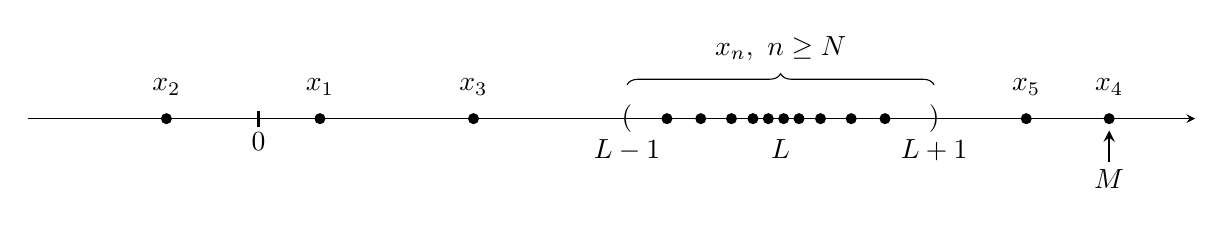
\begin{tikzpicture}[x=3.9cm,y=1cm]
  % Reta real, com seta stealth apenas no lado direito.
  \draw[-stealth] (-1.7,0) -- (2.1,0);

  % Origem usada apenas como referência visual.
  \draw[line width=0.8pt] (-0.95,-0.10) -- (-0.95,0.10)
    node[below=4pt] {$0$};

  % Intervalo aberto (L-1,L+1), com parêntesis centrados na reta.
  \node[anchor=center, inner sep=0pt] at (0.25,0) {$($};
  \node[anchor=center, inner sep=0pt] at (1.25,0) {$)$};
  \node[below=4pt] at (0.25,0) {$L-1$};
  \node[below=4pt] at (0.75,0) {$L$};
  \node[below=4pt] at (1.25,0) {$L+1$};

  % Chave para os termos que permanecem no intervalo.
  \draw[decorate, decoration={brace, amplitude=4pt}]
    (0.25,0.43) -- (1.25,0.43)
    node[midway, above=5pt] {$x_n,\ n\geq N$};

  % Termos anteriores ao N-ésimo termo.
  \fill (-1.25,0) circle (2pt) node[above=5pt] {$x_2$};
  \fill (-0.75,0) circle (2pt) node[above=5pt] {$x_1$};
  \fill (-0.25,0) circle (2pt) node[above=5pt] {$x_3$};

  % Termos a partir de N, mais aglutinados em torno de L.
  \foreach \x in {0.38,0.49,0.59,0.66,0.71,0.76,0.81,0.88,0.98,1.09} {
    \fill (\x,0) circle (2pt);
  }

  % Termos ainda não controlados pela escolha de N.
  \fill (1.55,0) circle (2pt) node[above=5pt] {$x_5$};
  \fill (1.82,0) circle (2pt) node[above=5pt] {$x_4$};
  \node[below=5pt] at (1.82,-0.35) {$M$};
  \draw[thick,-stealth] (1.82,-0.55) -- (1.82,-0.15);
\end{tikzpicture}
\end{center}

Ainda precisamos nos preocupar (levemente) com os termos da sequência 
que aparecem antes do $N$-ésimo termo. 
Como há apenas uma quantidade finita deles, tomamos
\[
M = \max\{|x_1|, |x_2|, |x_3|, \dots, |x_{N-1}|, |L| + 1\}.
\]
Segue-se que $|x_n| \leq M$ para todo $n \in \mathbb{N}$, como desejado.
\end{proof}

Este capítulo começou com uma demonstração de como a aplicação de propriedades algébricas familiares (comutatividade da adição) a objetos infinitos (séries) pode levar a resultados paradoxais. Esses exemplos destinam-se a incutir em nós um senso de cautela e a justificar o extremo cuidado que estamos tomando ao tirar nossas conclusões. Os teoremas a seguir ilustram que as sequências se comportam extremamente bem com respeito às operações de adição, multiplicação, divisão e ordem. \index[remissivo]{rearranjo}

\index[remissivo]{limites!propriedades algébricas}
\begin{theorem}[Propriedades Algébricas de Limites]\label{thm:limite-algebrico}
Sejam $\lim a_n = a$ e $\lim b_n = b$. Então,
\begin{enumerate}[label=(\roman*)]
\item $\lim (ca_n) = ca$, \quad para todo $c \in \mathbb{R}$;
\item $\lim (a_n + b_n) = a + b$;
\item $\lim (a_n b_n) = ab$;
\item $\lim (a_n / b_n) = a / b$, \ desde que $b \neq 0$.
\end{enumerate}
\end{theorem}

\begin{proof}
(i) Consideremos o caso em que $c \neq 0$. Queremos mostrar que a sequência $(ca_n)$ converge para $ca$, de modo que a estrutura da demonstração segue o modelo que descrevemos na \Cref{sec2:limite-sequencia}. Primeiro, seja $\varepsilon$ um número positivo arbitrário. Nosso objetivo é encontrar algum ponto na sequência $(ca_n)$ a partir do qual tenhamos
\[
|ca_n - ca| < \varepsilon.
\]
Ora,
\[
|ca_n - ca| = |c|\, |a_n - a|.
\]
Sabemos, por hipótese, que $(a_n) \to a$; logo, podemos tornar $|a_n - a|$ tão pequeno quanto quisermos. Em particular, podemos escolher $N$ tal que
\[
|a_n - a| < \frac{\varepsilon}{|c|}
\]
sempre que $n \geq N$. Para ver que este $N$ de fato funciona, observe que, para todo $n \geq N$,
\[
|ca_n - ca| = |c|\, |a_n - a| < |c| \, \frac{\varepsilon}{|c|} = \varepsilon.
\]
O caso $c = 0$ reduz-se a mostrar que a sequência constante $(0, 0, 0, \dots)$ converge para $0$, o que é facilmente verificado.

Antes de prosseguir com os itens (ii), (iii) e (iv), convém observar que a demonstração de (i), embora algo curta, é extremamente típica de uma prova de convergência. Antes de embarcar em um argumento formal, é uma boa ideia fazer um inventário daquilo que queremos tornar menor que $\varepsilon$ e daquilo que sabemos poder ser tornado pequeno para escolhas adequadas de $n$. Na demonstração anterior, queríamos tornar $|ca_n - ca| < \varepsilon$, e sabíamos que $|a_n - a|$ podia ser tornado \textit{tão pequeno quanto quiséssemos} (para valores grandes de $n$). Note que, em (i) e em todos os argumentos subsequentes, a estratégia é, a cada vez, majorar a quantidade que queremos tornar menor que $\varepsilon$ --- a qual, em cada caso, é
\[
|(\text{termos da sequência}) - (\text{limite proposto})|,
\]
--- por alguma combinação algébrica de quantidades sobre as quais temos controle.

(ii) Para provar esta afirmação, precisamos argumentar que a quantidade
\[
|(a_n + b_n) - (a + b)|
\]
pode ser tornada menor que um $\varepsilon$ arbitrário usando as hipóteses de que $|a_n - a|$ e $|b_n - b|$ podem ser tornados tão pequenos quanto quisermos para $n$ grande. O primeiro passo é usar a desigualdade triangular (\Cref{ex:desigualdade-triangular}) para obter \index[remissivo]{desigualdade triangular}
\[
|(a_n + b_n) - (a + b)| = |(a_n - a) + (b_n - b)| \leq |a_n - a| + |b_n - b|.
\]
Novamente, seja $\varepsilon > 0$ arbitrário. A técnica, desta vez, é dividir o $\varepsilon$ entre as duas expressões do lado direito da desigualdade acima. Usando a hipótese de que $(a_n) \to a$, sabemos que existe $N_1$ tal que
\[
|a_n - a| < \frac{\varepsilon}{2} \quad \text{sempre que} \quad n \geq N_1.
\]
Analogamente, a hipótese $(b_n) \to b$ nos permite escolher $N_2$ de modo que
\[
|b_n - b| < \frac{\varepsilon}{2} \quad \text{sempre que} \quad n \geq N_2.
\]
Surge então a questão de qual dos índices $N_1$ ou $N_2$ devemos tomar como nossa escolha de $N$. Escolhendo $N = \max\{N_1, N_2\}$, garantimos que, se $n \geq N$, então $n \geq N_1$ e $n \geq N_2$. Isso nos permite concluir que
\[
\begin{array}{rcl}
|(a_n + b_n) - (a + b)|
& \leq & |a_n - a| + |b_n - b| \\[2pt]
& < & \displaystyle\frac{\varepsilon}{2} + \frac{\varepsilon}{2} = \varepsilon
\end{array}
\]
para todo $n \geq N$, como desejado.

(iii) Para mostrar que $(a_n b_n) \to ab$, começamos observando que
\[
\begin{array}{rcl}
|a_n b_n - ab|
& = & |a_n b_n - ab_n + ab_n - ab| \\[2pt]
& \leq & |a_n b_n - ab_n| + |ab_n - ab| \\[2pt]
& = & |b_n|\, |a_n - a| + |a|\, |b_n - b|.
\end{array}
\]
Na primeira etapa, subtraímos e em seguida adicionamos $ab_n$, o que criou uma oportunidade de usar a desigualdade triangular. Essencialmente, quebramos a distância de $a_n b_n$ a $ab$ com um ponto intermediário e estamos usando a soma das duas distâncias para superestimar a distância original. Esse truque engenhoso tornar-se-á uma técnica familiar nos argumentos que virão. \index[remissivo]{desigualdade triangular}

Seja $\varepsilon > 0$ arbitrário e procedamos novamente com a estratégia de tornar cada parcela da desigualdade acima menor que $\varepsilon/2$. Para a parcela do lado direito ($|a|\,|b_n - b|$), se $a \neq 0$ podemos escolher $N_1$ de modo que
\[
n \geq N_1 \quad \text{implica} \quad |b_n - b| < \frac{1}{|a|} \frac{\varepsilon}{2}.
\]
(O caso $a = 0$ é tratado no \Cref{ex:2-3-9}.) Tornar a parcela do lado esquerdo $(|b_n|\,|a_n - a|)$ menor que $\varepsilon/2$ é complicado pelo fato de termos uma quantidade variável $|b_n|$ para lidar, em contraste com a constante $|a|$ que encontramos na parcela direita. A ideia é substituir $|b_n|$ por uma estimativa de pior caso. Usando o fato de que sequências convergentes são limitadas (\Cref{thm:convergente-limitada}), sabemos que existe uma cota $M > 0$ satisfazendo $|b_n| \leq M$ para todo $n \in \mathbb{N}$. Agora, podemos escolher $N_2$ de modo que
\[
|a_n - a| < \frac{1}{M} \frac{\varepsilon}{2} \quad \text{sempre que} \quad n \geq N_2.
\]
Para finalizar o argumento, tome $N = \max\{N_1, N_2\}$ e observe que, se $n \geq N$, então
\[
\begin{array}{rcl}
|a_n b_n - ab|
& \leq & |a_n b_n - ab_n| + |ab_n - ab| \\[2pt]
& = & |b_n|\, |a_n - a| + |a|\, |b_n - b| \\[2pt]
& \leq & M\, |a_n - a| + |a|\, |b_n - b| \\[2pt]
& < & M \left( \frac{\varepsilon}{2M} \right) + |a| \left( \frac{\varepsilon}{2|a|} \right) = \frac{\varepsilon}{2} + \frac{\varepsilon}{2} = \varepsilon.
\end{array}
\]

(iv) Esta última afirmação decorrerá de (iii) se conseguirmos provar que
\[
(b_n) \to b \quad \text{implica} \quad \left( \frac{1}{b_n} \right) \to \frac{1}{b}
\]
sempre que $b \neq 0$. Começamos observando que
\[
\left| \frac{1}{b_n} - \frac{1}{b} \right| = \frac{|b - b_n|}{|b|\,|b_n|}.
\]
Como $(b_n) \to b$, podemos tornar o numerador acima tão pequeno quanto quisermos escolhendo $n$ grande. O problema está em que precisamos de uma estimativa de pior caso para o tamanho de $1/(|b|\,|b_n|)$. Como os termos $b_n$ estão no denominador, não estamos mais interessados em uma cota superior para $|b_n|$, mas sim em uma desigualdade da forma $|b_n| \geq \delta > 0$. Isso nos dará então uma cota para o tamanho de $1/(|b|\,|b_n|)$.

O truque é olhar suficientemente adiante na sequência $(b_n)$ de modo que os termos estejam mais próximos de $b$ do que de $0$. Considere o valor particular $\varepsilon_0 = |b|/2$. Como $(b_n) \to b$, existe $N_1$ tal que $|b_n - b| < |b|/2$ para todo $n \geq N_1$. Isso implica $|b_n| > |b|/2$.

Em seguida, escolha $N_2$ de modo que $n \geq N_2$ implique
\[
|b_n - b| < \frac{\varepsilon |b|^2}{2}.
\]
Finalmente, se tomarmos $N = \max\{N_1, N_2\}$, então $n \geq N$ implica
\[
\left| \frac{1}{b_n} - \frac{1}{b} \right|
= |b - b_n| \, \frac{1}{|b|\,|b_n|}
< \frac{\varepsilon |b|^2}{2}\, \frac{1}{|b| \cdot \frac{|b|}{2}} = \varepsilon.
\]
\end{proof}

\subsection{Limites e Ordem}

Embora haja alguns perigos a evitar (veja o \Cref{ex:2-3-7}), o Teorema do Limite Algébrico verifica que a relação entre combinações algébricas de sequências e o processo de limite é tão livre de problemas quanto poderíamos esperar. Limites podem ser calculados a partir das sequências componentes individuais, desde que cada limite componente exista. O processo de limite também se comporta bem com respeito à operação de ordem.


\begin{theorem}\label{thm:limite-ordem}
Suponha que $\lim a_n = a$ e $\lim b_n = b$.
\begin{enumerate}[label=(\roman*)]
\item Se $a_n \geq 0$ para todo $n \in \mathbb{N}$, então $a \geq 0$.
\item Se $a_n \leq b_n$ para todo $n \in \mathbb{N}$, então $a \leq b$.
\item Se existe $c \in \mathbb{R}$ tal que $c \leq b_n$ para todo $n \in \mathbb{N}$, então $c \leq b$. Analogamente, se $a_n \leq c$ para todo $n \in \mathbb{N}$, então $a \leq c$.
\end{enumerate}
\end{theorem}

\begin{proof}
(i) Provaremos por contradição; suponhamos, portanto, que $a < 0$. A ideia é produzir um termo da sequência $(a_n)$ que também seja menor que zero. Para isso, consideremos o valor particular $\varepsilon = |a|$. A definição de convergência garante que podemos encontrar $N$ tal que $|a_n - a| < |a|$ para todo $n \geq N$. Em particular, isso significaria que $|a_N - a| < |a|$, o que implica $a_N < 0$. Isso contradiz nossa hipótese de que $a_N \geq 0$. Concluímos, portanto, que $a \geq 0$. \index[remissivo]{demonstração!por contradição}

% Ilustração geométrica da demonstração por contradição.
\begin{center}
\begin{tikzpicture}[x=4.2cm,y=1cm]
  % Reta real, com seta stealth apenas no lado direito.
  \draw[-stealth] (-1.7,0) -- (1.85,0);

  % Intervalo aberto (a-epsilon,0), com os parêntesis centrados na reta.
  \node[anchor=center, inner sep=0pt] at (-0.65,0) {$($};
  \node[anchor=center, inner sep=0pt] at (0.45,0) {$)$};
  \node[below=4pt] at (-0.65,0) {$a-\varepsilon$};
  \node[below=4pt] at (-0.10,0) {$a$};
  \node[below=4pt] at (0.62,0) {$0=a+\varepsilon$};

  % Pontos de referência e o termo que produz a contradição.
  \draw[line width=0.8pt] (-0.10,-0.10) -- (-0.10,0.10);

  % Termos que se aproximam de a pela direita.
  \foreach \x in {-0.07,-0.04,0,0.04,0.08} {
    \fill (\x,0) circle (2pt);
  }

  % Um termo ainda mais afastado de a, escolhido para a contradição.
  \fill (0.28,0) circle (2pt);
  \node[above=5pt] at (0.28,0.35) {$a_N$};
  \draw[thick,-stealth] (0.28,0.55) -- (0.28,0.15);

  % Os demais termos, não negativos, aparecem à direita de zero.
  \foreach \x in {0.64,0.84,1.04,1.24} {
    \fill (\x,0) circle (2pt);
  }
  \node[above=5pt] at (0.84,0) {$\cdots$};
  \node[above=5pt] at (1.04,0) {$a_2$};
  \node[above=5pt] at (1.24,0) {$a_1$};
\end{tikzpicture}
\end{center}

(ii) O Teorema do Limite Algébrico garante que a sequência $(b_n - a_n)$ converge para $b - a$. Como $b_n - a_n \geq 0$, podemos aplicar o item (i) para obter $b - a \geq 0$.

(iii) Tome $a_n = c$ (ou $b_n = c$) para todo $n \in \mathbb{N}$ e aplique (ii).
\end{proof}

Vale uma palavra sobre a ideia de ``caudas''. Grosso modo, os limites e suas propriedades não dependem em absoluto do que acontece no início da sequência, mas são estritamente determinados pelo que acontece quando $n$ se torna grande. Alterar o valor dos dez primeiros --- ou dos dez mil primeiros --- termos de uma sequência particular não tem efeito algum sobre o limite. O \Cref{thm:limite-ordem}, item~(i), por exemplo, supõe que $a_n \geq 0$ para \textit{todo} $n \in \mathbb{N}$. No entanto, a hipótese poderia ser enfraquecida supondo-se apenas que existe algum ponto $N_1$ a partir do qual $a_n \geq 0$ para todo $n \geq N_1$. O teorema permanece verdadeiro e, de fato, a mesma demonstração é válida, com a ressalva de que, quando $N$ for escolhido, ele seja pelo menos tão grande quanto $N_1$. \index[remissivo]{sequência!cauda}

Na linguagem da análise, quando uma propriedade (como a não-negatividade) não é necessariamente possuída por um número finito de termos iniciais, mas é possuída por todos os termos da sequência após um certo ponto $N$, dizemos que a sequência \textit{eventualmente} possui essa propriedade. (Veja o \Cref{ex:2-2-7}.) O \Cref{thm:limite-ordem}, item~(i), poderia ser reformulado como: ``sequências convergentes que são eventualmente não-negativas convergem para limites não-negativos.'' Os itens~(ii) e (iii) admitem modificações análogas, assim como muitos outros resultados que virão.

\subsection{Lista de Exercícios}\label{subsec:exercicios-teoremas-limite}

\begin{exercise}\label{ex:2-3-1}
Seja $x_n \geq 0$ para todo $n \in \mathbb{N}$.
\begin{enumerate}[label=(\alph*)]
\item Se $(x_n) \to 0$, mostre que $(\sqrt{x_n}) \to 0$.
\item Se $(x_n) \to x$, mostre que $(\sqrt{x_n}) \to \sqrt{x}$.
\end{enumerate}
\end{exercise}

\begin{exercise}\label{ex:2-3-2}
Usando apenas a \Cref{def:convergencia-sequencia}, prove que, se $(x_n) \to 2$, então
\begin{enumerate}[label=(\alph*)]
\item $\displaystyle \left( \frac{2x_n - 1}{3} \right) \to 1$;
\item $(1 / x_n) \to 1/2$.
\end{enumerate}
(evite usar as propriedades algébricas de limites)
\end{exercise}

\begin{exercise}[Teorema do Confronto]\label{ex:2-3-3}
Mostre que, se $x_n \leq y_n \leq z_n$ para todo $n \in \mathbb{N}$, e se $\lim x_n = \lim z_n = l$, então $\lim y_n = l$ também.
\end{exercise}

\begin{exercise}\label{ex:2-3-4}
Seja $(a_n) \to 0$ e use o Teorema do Limite Algébrico para calcular cada um dos limites a seguir (supondo que as frações estejam sempre definidas):
\begin{enumerate}[label=(\alph*)]
\item $\displaystyle \lim \left( \frac{1 + 2a_n}{1 + 3a_n - 4a_n^2} \right)$
\item $\displaystyle \lim \left( \frac{(a_n + 2)^2 - 4}{a_n} \right)$
\item $\displaystyle \lim \left( \frac{\frac{2}{a_n} + 3}{\frac{1}{a_n} + 5} \right)$.
\end{enumerate}
\end{exercise}

\begin{exercise}\label{ex:2-3-5}
Sejam $(x_n)$ e $(y_n)$ dadas e defina $(z_n)$ como a sequência ``embaralhada''
\[
(x_1, y_1, x_2, y_2, x_3, y_3, \dots, x_n, y_n, \dots).
\]
Prove que $(z_n)$ é convergente se, e somente se, $(x_n)$ e $(y_n)$ são ambas convergentes com $\lim x_n = \lim y_n$.
\end{exercise}

\begin{exercise}\label{ex:2-3-6}
Considere a sequência dada por $b_n = n - \sqrt{n^2 + 2n}$. Tomando $(1/n) \to 0$ como dado e usando tanto o Teorema do Limite Algébrico quanto o resultado do \Cref{ex:2-3-1}, mostre que $\lim b_n$ existe e encontre o valor do limite.
\end{exercise}

\begin{exercise}\label{ex:2-3-7}
Dê um exemplo de cada um dos itens a seguir, ou afirme que tal pedido é impossível, referenciando o(s) teorema(s) apropriado(s):
\begin{enumerate}[label=(\alph*)]
\item sequências $(x_n)$ e $(y_n)$, ambas divergentes, mas cuja soma $(x_n + y_n)$ converge;
\item sequências $(x_n)$ e $(y_n)$ em que $(x_n)$ converge, $(y_n)$ diverge e $(x_n + y_n)$ converge;
\item uma sequência convergente $(b_n)$ com $b_n \neq 0$ para todo $n$, tal que $(1/b_n)$ diverge;
\item uma sequência ilimitada $(a_n)$ e uma sequência convergente $(b_n)$ com $(a_n - b_n)$ limitada;
\item duas sequências $(a_n)$ e $(b_n)$ em que $(a_n b_n)$ e $(a_n)$ convergem, mas $(b_n)$ não converge.
\end{enumerate}
\end{exercise}

\begin{exercise}\label{ex:2-3-8}
Sejam $(x_n) \to x$ e $p(x)$ um polinômio.
\begin{enumerate}[label=(\alph*)]
\item Mostre que $p(x_n) \to p(x)$.
\item Dê um exemplo de uma função $f(x)$ e de uma sequência convergente $(x_n) \to x$ em que a sequência $f(x_n)$ converge, mas não para $f(x)$.
\end{enumerate}
\end{exercise}

\bigskip 

\begin{exercise}\label{ex:2-3-9}
\begin{enumerate}[label=(\alph*)]
\item Seja $(a_n)$ uma sequência!limitada (não necessariamente convergente) e suponha que $\lim b_n = 0$. Mostre que $\lim(a_n b_n) = 0$. Por que não podemos usar o Teorema do Limite Algébrico para provar isso?
\item Podemos concluir algo sobre a convergência de $(a_n b_n)$ se supusermos que $(b_n)$ converge para algum limite não-nulo $b$?
\item Use (a) para provar o \Cref{thm:limite-algebrico}, item~(iii), para o caso em que $a = 0$.
\end{enumerate}
\end{exercise}

\begin{exercise}\label{ex:2-3-10}
Considere a lista de conjecturas a seguir. Forneça uma demonstração curta para as que são verdadeiras e um contraexemplo para qualquer uma que seja falsa.
\begin{enumerate}[label=(\alph*)]
\item Se $\lim(a_n - b_n) = 0$, então $\lim a_n = \lim b_n$.
\item Se $(b_n) \to b$, então $|b_n| \to |b|$.
\item Se $(a_n) \to 0$ e $(b_n - a_n) \to 0$, então $(b_n) \to a$.
\item Se $(a_n) \to 0$ e $|b_n - b| \leq a_n$ para todo $n \in \mathbb{N}$, então $(b_n) \to b$.
\end{enumerate}
\end{exercise}

\index[remissivo]{média de Cesàro}
\begin{exercise}[Médias de Cesàro]\label{ex:2-3-11}
\begin{enumerate}[label=(\alph*)]
\item Mostre que, se $(x_n)$ é uma sequência convergente, então a sequência dada pelas médias
\[
y_n = \frac{x_1 + x_2 + \cdots + x_n}{n}
\]
também converge para o mesmo limite.
\item Dê um exemplo para mostrar que é possível que a sequência $(y_n)$ das médias convirja mesmo que $(x_n)$ não convirja.
\end{enumerate}
\end{exercise}

\begin{exercise}\label{ex:2-3-12}
Uma tarefa típica em análise é decifrar se uma propriedade possuída por todo termo de uma sequência convergente é necessariamente herdada pelo limite. Suponha que $(a_n) \to a$ e determine a validade de cada afirmação. Tente produzir um contraexemplo para qualquer uma que seja falsa.
\begin{enumerate}[label=(\alph*)]
\item Se todo $a_n$ é uma cota superior para um conjunto $B$, então $a$ também é uma cota superior para $B$.
\item Se todo $a_n$ está no complementar do intervalo $(0, 1)$, então $a$ também está no complementar de $(0, 1)$.
\item Se todo $a_n$ é racional, então $a$ é racional.
\end{enumerate}
\end{exercise}

\begin{exercise}[Limites Iterados]\label{ex:2-3-13}
Dada uma família duplamente indexada $a_{mn}$, em que $m, n \in \mathbb{N}$, o que deveria representar $\displaystyle \lim_{m,n \to \infty} a_{mn}$?
\begin{enumerate}[label=(\alph*)]
\item Seja $a_{mn} = m/(m + n)$ e compute os limites iterados
\[
\lim_{n \to \infty} \Bigl( \lim_{m \to \infty} a_{mn} \Bigr) \quad \text{e} \quad
\lim_{m \to \infty} \Bigl( \lim_{n \to \infty} a_{mn} \Bigr).
\]
Defina $\displaystyle \lim_{m,n \to \infty} a_{mn} = a$ como significando que, para todo $\varepsilon > 0$, existe $N \in \mathbb{N}$ tal que, se ambos $m, n \geq N$, então $|a_{mn} - a| < \varepsilon$.
\item Seja $a_{mn} = 1/(m + n)$. O limite $\displaystyle \lim_{m,n \to \infty} a_{mn}$ existe neste caso? Os dois limites iterados existem? Como se comparam esses três valores? Responda às mesmas perguntas para $a_{mn} = mn/(m^2 + n^2)$.
\item Produza um exemplo em que $\displaystyle \lim_{m,n \to \infty} a_{mn}$ existe, mas nenhum dos dois limites iterados pode ser calculado.
\item Suponha que $\displaystyle \lim_{m,n \to \infty} a_{mn} = a$ e que, para cada $m \in \mathbb{N}$ fixado, $\displaystyle \lim_{n \to \infty} a_{mn} = b_m$. Mostre que $\displaystyle \lim_{m \to \infty} b_m = a$.
\item Prove que, se $\displaystyle \lim_{m,n \to \infty} a_{mn}$ existe e os dois limites iterados existem, então todos os três limites devem ser iguais.
\end{enumerate}
\end{exercise}

% ---------------------------------------------------------------------
% Seção 2.4 — O Teorema da Convergência Monótona e um Primeiro Olhar
% sobre Séries Infinitas
% (tradução para PT-BR de Abbott, Understanding Analysis, 2ª ed.,
% páginas 67–72 do OCR).
% ---------------------------------------------------------------------

\section[O Teorema de Convergência de Sequências Monótonas]
{Convergência de Sequências Monótonas e um\\ Primeiro Olhar sobre Séries Infinitas}\label{sec2:convergencia-monotona-series}

Mostramos no \Cref{thm:convergente-limitada} que sequências convergentes são limitadas. A recíproca certamente não é verdadeira. Não é difícil produzir um exemplo de uma sequência!limitada que não converge. Por outro lado, se uma sequência!limitada é monótona, então ela de fato converge.

\index[remissivo]{sequência!monótona} \index[remissivo]{sequência!monótona!crescente} \index[remissivo]{sequência!monótona!decrescente}
\begin{definition}[sequência monótona]\label{def:sequencia-monotona}
Uma sequência $(a_n)$ é \textit{crescente} se $a_n \leq a_{n+1}$ para todo $n \in \mathbb{N}$, e \textit{decrescente} se $a_n \geq a_{n+1}$ para todo $n \in \mathbb{N}$. Uma sequência é \textit{monótona} se é crescente ou decrescente.
\end{definition}

\index[remissivo]{teorema!da Convergência Monótona}
\begin{theorem}[Teorema da Convergência Monótona]\label{thm:convergencia-monotona}
Se uma sequência é monótona e limitada, então ela converge.
\end{theorem}

\begin{proof}
Seja $(a_n)$ monótona e limitada. Para provar que $(a_n)$ converge usando a definição de convergência, precisaremos de um candidato a limite. Suponhamos que a sequência seja crescente (o caso decrescente é tratado de maneira semelhante) e consideremos o conjunto $\{a_n : n \in \mathbb{N}\}$. Por hipótese, esse conjunto é limitado; portanto, podemos tomar
\[
\index[remissivo]{supremo!definição}
s = \sup\{a_n : n \in \mathbb{N}\}.
\]
É razoável afirmar que $\lim a_n=s$.

% Gráfico de uma sequência crescente convergindo para o seu supremo.
\begin{center}
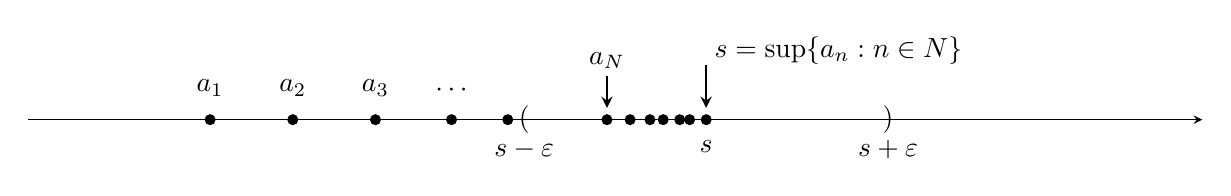
\begin{tikzpicture}[x=4.2cm,y=1cm]
  % Reta real, com seta stealth apenas no lado direito.
  \draw[-stealth] (-1.7,0) -- (1.85,0);

  % Intervalo de referência em torno do supremo.
  \node[anchor=center, inner sep=0pt] at (-0.20,0) {$($};
  \node[anchor=center, inner sep=0pt] at (0.90,0) {$)$};
  \node[below=4pt] at (-0.20,0) {$s-\varepsilon$};
  \node[below=4pt] at (0.35,0) {$s$};
  \node[below=4pt] at (0.90,0) {$s+\varepsilon$};

  % Ponto que representa o supremo.
  \fill (0.35,0) circle (2pt);
  \node[above=5pt] at (0.75,0.40)
    {$s=\sup\{a_n:n\in\mathbb{N}\}$};
  \draw[thick,-stealth] (0.35,0.7) -- (0.35,0.15);

  % Termos iniciais da sequência crescente.
  \foreach \x in {-1.15,-0.90,-0.65,-0.42,-0.25} {
    \fill (\x,0) circle (2pt);
  }
  \node[above=5pt] at (-1.15,0) {$a_1$};
  \node[above=5pt] at (-0.90,0) {$a_2$};
  \node[above=5pt] at (-0.65,0) {$a_3$};
  \node[above=5pt] at (-0.42,0) {$\cdots$};

  % A partir de a_N, os termos permanecem próximos de s.
  \fill (0.05,0) circle (2pt);
  \node[above=5pt] at (0.05,0.35) {$a_N$};
  \draw[thick,-stealth] (0.05,0.55) -- (0.05,0.15);
  \foreach \x in {0.12,0.18,0.22,0.27,0.30} {
    \fill (\x,0) circle (2pt);
  }
\end{tikzpicture}
\end{center}

Para provar isso, seja $\epsilon>0$. Como $s$ é a menor cota superior de $\{a_n:n\in\mathbb{N}\}$, $s-\epsilon$ não é uma cota superior; logo, existe um termo $a_N$ da sequência tal que $s-\epsilon<a_N$. Agora, o fato de $(a_n)$ ser crescente implica que, se $n\geq N$, então $a_N\leq a_n$. Consequentemente, \index[remissivo]{supremo!caracterização por $\varepsilon$}
\[
s-\epsilon<a_N\leq a_n\leq s<s+\epsilon,
\]
o que implica $|a_n-s|<\epsilon$, como desejado.
\end{proof}

O Teorema da Convergência Monótona é extremamente útil no estudo de séries infinitas, em grande parte porque afirma a convergência de uma sequência sem mencionar explicitamente qual é o limite. Este é um bom momento para algumas investigações preliminares; portanto, é hora de formalizar a relação entre sequências e séries.

\index[remissivo]{convergência} \index[remissivo]{série!infinita} \index[remissivo]{série!infinita!somas parciais} \index[remissivo]{soma!parcial}
\begin{definition}[Convergência de uma série]\label{def:convergencia-serie}
Seja $(b_n)$ uma sequência. Uma \textit{série infinita} é uma expressão formal da forma
\[
\sum_{n=1}^{\infty}b_n=b_1+b_2+b_3+b_4+b_5+\cdots.
\]
Definimos a sequência correspondente de \textit{somas parciais} $(s_m)$ por
\[
s_m=b_1+b_2+b_3+\cdots+b_m,
\]
e dizemos que a série $\sum_{n=1}^{\infty}b_n$ \textit{converge para $B$} se a sequência $(s_m)$ converge para $B$. Nesse caso, escrevemos $\sum_{n=1}^{\infty}b_n=B$.
\end{definition}

\begin{example}[Uma série de termos positivos]\label{exmpl:2-4-4}
Considere
\[
\sum_{n=1}^{\infty}\frac{1}{n^2}.
\]
Como todos os termos da soma são positivos, a sequência de somas parciais
\[
s_m=1+\frac14+\frac19+\cdots+\frac{1}{m^2}
\]
é crescente. A questão é saber se podemos encontrar uma cota superior para $(s_m)$. Para isso, observe que
\[
\begin{aligned}
s_m&=1+\frac{1}{2\cdot2}+\frac{1}{3\cdot3}+\frac{1}{4\cdot4}+\cdots+\frac{1}{m^2}\\
&<1+\frac{1}{2\cdot1}+\frac{1}{3\cdot2}+\frac{1}{4\cdot3}+\cdots+\frac{1}{m(m-1)}\\
&=1+\left(1-\frac12\right)+\left(\frac12-\frac13\right)+\left(\frac13-\frac14\right)+\cdots+\left(\frac{1}{m-1}-\frac1m\right)\\
&=1+1-\frac1m<2.
\end{aligned}
\]
Assim, $2$ é uma cota superior para a sequência de somas parciais. Pelo Teorema da Convergência Monótona, $\sum_{n=1}^{\infty}1/n^2$ converge para algum limite, desconhecido por enquanto, menor que $2$. (Encontrar o valor desse limite é o tema das Seções 6.1 e 8.3.) \index[remissivo]{cota!superior!conjunto limitado superiormente}
\end{example}

\index[remissivo]{série!harmônica}
\begin{example}[A série harmônica]\label{exmpl:2-4-5}
Desta vez, considere a chamada \textit{série harmônica}
\[
\sum_{n=1}^{\infty}\frac1n.
\]
Novamente, temos uma sequência crescente de somas parciais,
\[
s_m=1+\frac12+\frac13+\cdots+\frac1m,
\]
que, numa inspeção superficial, parece talvez ser limitada. Entretanto, $2$ já não é uma cota superior, pois
\[
s_4=1+\frac12+\left(\frac13+\frac14\right)>1+\frac12+\left(\frac14+\frac14\right)=2.
\]
Um cálculo semelhante mostra que $s_8>2\frac12$, e, em geral,
\[
\begin{aligned}
s_{2^k}&=1+\frac12+\left(\frac13+\frac14\right)+\left(\frac15+\cdots+\frac18\right)+\cdots\\
&\quad+\left(\frac{1}{2^{k-1}+1}+\cdots+\frac{1}{2^k}\right)\\
&>1+\frac12+2\left(\frac14\right)+4\left(\frac18\right)+\cdots+2^{k-1}\left(\frac{1}{2^k}\right)\\
&=1+\frac12+\frac12+\frac12+\cdots+\frac12=1+k\left(\frac12\right),
\end{aligned}
\]
que é ilimitada. Assim, apesar do ritmo incrivelmente lento, a sequência de somas parciais de $\sum_{n=1}^{\infty}1/n$ eventualmente ultrapassa qualquer número da reta real positiva. Como sequências convergentes são limitadas, a série harmônica diverge. \index[remissivo]{divergência}
\end{example}

O exemplo anterior é um caso particular de um argumento geral que pode ser usado para determinar a convergência ou divergência de uma grande classe de séries infinitas.

\index[remissivo]{teste!da Condensação de Cauchy}
\begin{theorem}[Teste da Condensação de Cauchy]\label{thm:condensacao-cauchy}
Suponha que $(b_n)$ seja decrescente e satisfaça $b_n\geq0$ para todo $n\in\mathbb{N}$. Então, a série $\sum_{n=1}^{\infty}b_n$ converge se, e somente se, a série
\[
\sum_{n=0}^{\infty}2^n b_{2^n}=b_1+2b_2+4b_4+8b_8+16b_{16}+\cdots
\]
converge.
\end{theorem}

\begin{proof}
Primeiro, suponha que $\sum_{n=0}^{\infty}2^n b_{2^n}$ converge. O \Cref{thm:convergente-limitada} garante que as somas parciais
\[
t_k=b_1+2b_2+4b_4+\cdots+2^k b_{2^k}
\]
são limitadas; isto é, existe $M>0$ tal que $t_k\leq M$ para todo $k\in\mathbb{N}$. Queremos provar que $\sum_{n=1}^{\infty}b_n$ converge. Como $b_n\geq0$, sabemos que as somas parciais são crescentes; basta, portanto, mostrar que
\[
s_m=b_1+b_2+b_3+\cdots+b_m
\]
é limitada.

Fixe $m$ e escolha $k$ suficientemente grande para garantir $m\leq2^{k+1}-1$. Então 
temos que 
$$s_m\leq s_{2^{k+1}-1}$$ 
e além do mais, segue da monotonicidade de $(b_n)$ que 
\[
\begin{aligned}
s_{2^{k+1}-1}&=b_1+(b_2+b_3)+(b_4+b_5+b_6+b_7)+\cdots +(b_{2^k}+\cdots+b_{2^{k+1}-1})
\\[0.3cm]
&\leq b_1+(b_2+b_2)+(b_4+b_4+b_4+b_4)+\cdots +(b_{2^k}+\cdots+b_{2^k})
\\[0.3cm]
&=b_1+2b_2+4b_4+\cdots+2^k b_{2^k}=t_k.
\end{aligned}
\]
Assim, $s_m\leq t_k\leq M$, e a sequência $(s_m)$ é limitada. Pelo Teorema de 
convergência de sequências monótonas, concluímos que $\sum_{n=1}^{\infty}b_n$ converge.

A demonstração de que a divergência de $\sum_{n=0}^{\infty}2^n b_{2^n}$ implica a divergência de $\sum_{n=1}^{\infty}b_n$ é semelhante à do \Cref{exmpl:2-4-5}. Os detalhes são pedidos no \Cref{ex:2-4-9}.
\end{proof}

\index[remissivo]{série!$p$-séries}
\begin{corollary}[$p$-Séries]\label{cor:serie-p}
A série $\displaystyle\sum_{n=1}^{\infty}\frac{1}{n^p}$ converge se, e somente se, $p>1$.
\end{corollary}

Uma demonstração rigorosa desse corolário requer alguns fatos básicos sobre séries geométricas. A demonstração é pedida no \Cref{ex:2-7-5}, ao final da \Cref{sec2:propriedades-series}, onde as séries geométricas são discutidas.

\subsection{Lista de Exercícios}\label{subsec:exercicios-convergencia-monotona}

\begin{exercise}\label{ex:2-4-1}
\begin{enumerate}[label=\alph*)]
\item Prove que a sequência definida por $x_1=3$ e $x_{n+1}=1/(4-x_n)$ converge.
\item Agora que sabemos que $\lim x_n$ existe, explique por que $\lim x_{n+1}$ também deve existir e ser igual ao mesmo valor.
\item Tome o limite de cada lado da equação recursiva do item (a) para calcular explicitamente $\lim x_n$.
\end{enumerate}
\end{exercise}

\begin{exercise}\label{ex:2-4-2}
\begin{enumerate}[label=\alph*)]
\item Considere a sequência definida recursivamente por $y_1=1$ e $y_{n+1}=3-y_n$, e escreva $y=\lim y_n$. Como $(y_n)$ e $(y_{n+1})$ têm o mesmo limite, tomar o limite na equação recursiva dá $y=3-y$. Resolvendo para $y$, concluímos que $\lim y_n=3/2$. O que há de errado nesse argumento?
\item Agora tome $y_1=1$ e $y_{n+1}=3-1/y_n$. A estratégia do item (a) pode ser aplicada para calcular o limite dessa sequência?
\end{enumerate}
\end{exercise}

\begin{exercise}\label{ex:2-4-3}
\begin{enumerate}[label=\alph*)]
\item Mostre que $\sqrt2,\sqrt{2+\sqrt2},\sqrt{2+\sqrt{2+\sqrt2}},\ldots$ converge e encontre o limite.
\item A sequência $\sqrt2,\sqrt{2\sqrt2},\sqrt{2\sqrt{2\sqrt2}},\ldots$ converge? Em caso afirmativo, encontre o limite.
\end{enumerate}
\end{exercise}

\begin{exercise}\label{ex:2-4-4}
\begin{enumerate}[label=\alph*)]
\item Na \Cref{sec:consequencias-completude} usamos o ``Axioma da Completude'' para provar a Propriedade Arquimediana de $\mathbb{R}$ (\Cref{thm:propriedade-arquimediana}). Mostre que o Teorema da Convergência Monótona também pode ser usado para provar a Propriedade Arquimediana sem fazer nenhum uso do Axioma da Completude.
\item Use o Teorema da Convergência Monótona para fornecer uma demonstração da Propriedade dos Intervalos Encaixados (\Cref{thm:intervalos-encaixados}) que não faça uso do Axioma da Completude.
\end{enumerate}
Esses dois resultados sugerem que poderíamos ter usado o Teorema da Convergência Monótona no lugar do Axioma da Completude como axioma inicial para construir uma teoria adequada dos números reais.
\end{exercise}

\begin{exercise}[Calculando Raízes Quadradas]\label{ex:2-4-5}
Seja $x_1=2$ e defina $x_{n+1}=\frac12\left(x_n+\frac2{x_n}\right)$.
\begin{enumerate}[label=\alph*)]
\item Mostre que $x_n^2\geq2$ sempre e use isso para provar que $x_n-x_{n+1}\geq0$. Conclua que $\lim x_n=\sqrt2$.
\item Modifique a sequência $(x_n)$ de modo que ela convirja para $\sqrt c$.
\end{enumerate}
\end{exercise}

\begin{exercise}[Média Aritmético-Geométrica]\label{ex:2-4-6}
\begin{enumerate}[label=\alph*)]
\item Explique por que $\sqrt{xy}\leq(x+y)/2$ para quaisquer dois números reais positivos $x$ e $y$. (A média geométrica é sempre menor ou igual à média aritmética.)
\item Se $0\leq x_1\leq y_1$, defina $x_{n+1}=\sqrt{x_ny_n}$ e $y_{n+1}=(x_n+y_n)/2$. Mostre que $\lim x_n$ e $\lim y_n$ existem e são iguais.
\end{enumerate}
\end{exercise}

\begin{exercise}[Limite Superior]\label{ex:2-4-7}
Seja $(a_n)$ uma sequência limitada.
\begin{enumerate}[label=\alph*)]
\item Prove que a sequência $y_n=\sup\{a_k:k\geq n\}$ converge.
\item O limite superior de $(a_n)$, ou $\limsup a_n$, é definido 
por $\limsup a_n=\lim y_n$, em que $(y_n)$ é a sequência do item (a). 
Dê uma definição razoável para $\liminf a_n$ 
e explique brevemente por que ele sempre existe para toda sequência limitada.
\item Prove que $\liminf a_n\leq\limsup a_n$ para toda sequência limitada 
e dê um exemplo de sequência para a qual a desigualdade é estrita.
\item Mostre que $\liminf a_n=\limsup a_n$ se, e somente se, $\lim a_n$ existe. Nesse caso, os três valores são iguais.
\end{enumerate}
\end{exercise}

\begin{exercise}\label{ex:2-4-8}
Para cada série, encontre uma fórmula explícita para a sequência de somas parciais e determine se a série converge.
\begin{enumerate}[label=\alph*)]
\item $\displaystyle\sum_{n=1}^{\infty}\frac1{2^n}$;
\item $\displaystyle\sum_{n=1}^{\infty}\frac1{n(n+1)}$;
\item $\displaystyle\sum_{n=1}^{\infty}\log\left(\frac{n+1}{n}\right)$.
\end{enumerate}
No item (c), $\log(x)$ refere-se à função logaritmo natural do cálculo.
\end{exercise}

\begin{exercise}\label{ex:2-4-9}
Complete a demonstração do \Cref{thm:condensacao-cauchy}, mostrando que, se a série $\sum_{n=0}^{\infty}2^n b_{2^n}$ diverge, então $\sum_{n=1}^{\infty}b_n$ também diverge. O \Cref{exmpl:2-4-5} pode ser uma referência útil.
\end{exercise}

\index[remissivo]{produto!infinito}
\begin{exercise}[Produtos Infinitos]\label{ex:2-4-10}
Um parente próximo das séries infinitas é o produto infinito
\[
\prod_{n=1}^{\infty}b_n=b_1b_2b_3\cdots,
\]
que é entendido em termos de sua sequência de produtos parciais \index[remissivo]{produto!infinito!produtos parciais}
\[
p_m=\prod_{n=1}^{m}b_n=b_1b_2b_3\cdots b_m.
\]
Considere a classe especial de produtos infinitos da forma
\[
\prod_{n=1}^{\infty}(1+a_n)=(1+a_1)(1+a_2)(1+a_3)\cdots,
\]
em que $a_n\geq0$.
\begin{enumerate}[label=\alph*)]
\item Encontre uma fórmula explícita para a sequência de produtos parciais no caso em que $a_n=1/n$ e decida se a sequência converge. Escreva os primeiros termos da sequência de produtos parciais no caso em que $a_n=1/n^2$ e formule uma conjectura sobre a convergência dessa sequência.
\item Mostre, em geral, que a sequência de produtos parciais converge se, e somente se, $\sum_{n=1}^{\infty}a_n$ converge. (A desigualdade $1+x\leq3^x$ para $x$ positivo será útil em uma das direções.)
\end{enumerate}
\end{exercise}

% ---------------------------------------------------------------------
% Seção 2.5 — Subsequências e o Teorema de Bolzano--Weierstrass
% (tradução para PT-BR de Abbott, Understanding Analysis, 2ª ed.,
% páginas 73–77 do OCR).
% ---------------------------------------------------------------------

\section{Subsequências e o Teorema de Bolzano--Weierstrass}\label{sec2:subsequencias-bolzano-weierstrass}

No \Cref{exmpl:2-4-5}, mostramos que a sequência de somas parciais $(s_m)$ da série harmônica não converge concentrando nossa atenção em uma subsequência particular $(s_{2^k})$ da sequência original. No momento, deixaremos de lado o tópico de séries infinitas e desenvolveremos mais plenamente o importante conceito de subsequências.

\index[remissivo]{subsequência}
\begin{definition}\label{def:subsequencia}
Seja $(a_n)$ uma sequência de números reais, e seja $n_1 < n_2 < n_3 < n_4 < n_5 < \cdots$ uma sequência crescente de números naturais. Então a sequência
\[
(a_{n_1}, a_{n_2}, a_{n_3}, a_{n_4}, a_{n_5}, \dots)
\]
é chamada de \textit{subsequência} de $(a_n)$ e é denotada por $(a_{n_k})$, onde $k \in \mathbb{N}$ indexa a subsequência. \index[remissivo]{subsequência!convergente}
\end{definition}

Observe que a ordem dos termos em uma subsequência é a mesma que na sequência original, e repetições não são permitidas. Assim, se
\[
(a_n) = \Bigl(1, \frac12, \frac13, \frac14, \frac15, \frac16, \dots \Bigr),
\]
então
\[
\Bigl( \frac12, \frac14, \frac16, \frac18, \dots \Bigr)
\quad\text{e}\quad
\Bigl( \frac{1}{10}, \frac{1}{100}, \frac{1}{1000}, \frac{1}{10000}, \dots \Bigr)
\]
são exemplos de subsequências legítimas, enquanto
\[
\Bigl( \frac{1}{10}, \frac15, \frac{1}{100}, \frac{1}{50}, \frac{1}{1000}, \frac{1}{500}, \dots \Bigr)
\quad\text{e}\quad
\Bigl( 1, 1, \frac13, \frac13, \frac15, \frac15, \dots \Bigr)
\]
não o são.

\index[remissivo]{subsequência!convergente}
\begin{theorem}\label{thm:subsequencias-convergentes}
\textit{Subsequências de uma sequência convergente convergem para o mesmo limite da sequência original.}
\end{theorem}

\begin{proof}
Suponha que $(a_n) \to a$, e seja $(a_{n_k})$ uma subsequência. Dado $\varepsilon > 0$, existe $N$ tal que $|a_n - a| < \varepsilon$ sempre que $n \geq N$. Como $n_k \geq k$ para todo $k$, o mesmo $N$ servirá para a subsequência; isto é, $|a_{n_k} - a| < \varepsilon$ sempre que $k \geq N$.
\end{proof}

Este resultado pouco surpreendente tem várias aplicações algo surpreendentes. Ele é o ingrediente chave para entender quando somas infinitas são associativas (\Cref{ex:2-5-3}). Também podemos usá-lo da seguinte maneira engenhosa para calcular valores de alguns limites familiares.

\begin{example}\label{exmpl:2-5-3}
Seja $0 < b < 1$. Como
\[
b > b^2 > b^3 > b^4 > \dots > 0,
\]
a sequência $(b^n)$ é decrescente e limitada inferiormente. O Teorema da Convergência Monótona (\Cref{thm:convergencia-monotona}) nos permite concluir que $(b^n)$ converge para algum $l$ satisfazendo $b > l \geq 0$. Para calcular $l$, observe que $(b^{2n})$ é uma subsequência, logo $(b^{2n}) \to l$ pelo \Cref{thm:subsequencias-convergentes}. Mas $b^{2n} = b^n \cdot b^n$, portanto, 
segue das propriedades algébricas de limites provadas no   
\Cref{thm:limite-algebrico} que $(b^{2n}) \to l \cdot l = l^2$. Como os limites são únicos (\Cref{thm:unicidade-limite}), $l^2 = l$ e, portanto, $l = 0$.
\end{example}

Sem muita dificuldade (\Cref{ex:2-5-7}), podemos generalizar este exemplo para concluir que $(b^n) \to 0$ se, e somente se, $-1 < b < 1$.

\index[remissivo]{divergência}
\begin{example}[Critério de Divergência]\label{exmpl:2-5-4}
O \Cref{thm:subsequencias-convergentes} também é útil para fornecer demonstrações econômicas de divergência. No \Cref{exmpl:2-2-8}, estávamos razoavelmente certos de que
\[
\Bigl( 1, -\frac12, \frac13, -\frac14, \frac15, -\frac15, \frac15, -\frac15, \frac15, -\frac15, \frac15, -\frac15, \frac15, -\frac15, \dots \Bigr)
\]
não convergia para nenhum limite proposto. Observe que
\[
\Bigl( \frac15, \frac15, \frac15, \frac15, \frac15, \dots \Bigr)
\]
é uma subsequência que converge para $1/5$. Além disso,
\[
\Bigl( -\frac15, -\frac15, -\frac15, -\frac15, -\frac15, \dots \Bigr)
\]
é uma subsequência diferente da sequência original que converge para $-1/5$. Como temos duas subsequências convergindo para dois limites distintos, podemos concluir rigorosamente que a sequência original diverge.
\end{example}

\subsection{O Teorema de Bolzano--Weierstrass}

No exemplo anterior, foi bastante fácil identificar uma subsequência convergente (ou duas) escondida na sequência original. Para sequências limitadas, verifica-se que é sempre possível encontrar pelo menos uma tal subsequência convergente.

\index[remissivo]{teorema!de Bolzano--Weierstrass}
\begin{theorem}[Teorema de Bolzano--Weierstrass]\label{thm:bolzano-weierstrass}
\textit{Toda sequência limitada contém uma subsequência convergente.}
\end{theorem}

\begin{proof}
Seja $(a_n)$ uma sequência limitada, de modo que existe $M > 0$ satisfazendo $|a_n| \leq M$ para todo $n \in \mathbb{N}$. Bisseccione o intervalo fechado $[-M, M]$ em dois intervalos fechados $[-M, 0]$ e $[0, M]$. (O ponto médio está incluído em ambas as metades.) Agora, necessariamente pelo menos um desses intervalos fechados contém uma quantidade infinita de termos da sequência $(a_n)$. Selecione uma metade para a qual isso ocorre e denote esse intervalo por $I_1$. Em seguida, seja $a_{n_1}$ algum termo da sequência $(a_n)$ satisfazendo $a_{n_1} \in I_1$.

% Construção dos intervalos encaixados $I_1$ e $I_2$.
\begin{center}
\begin{tikzpicture}[x=4.2cm,y=1cm]
  % Intervalo inicial limitado e reta real.
  \draw[-stealth] (-1.7,0) -- (1.85,0);
  \draw[line width=0.8pt] (-1.5,-0.10) -- (-1.5,0.10)
    node[below=4pt] {$-M$};
  \draw[line width=0.8pt] (0,-0.10) -- (0,0.10) node[below=4pt] {$0$};
  \draw[line width=0.8pt] (1.5,-0.10) -- (1.5,0.10)
    node[below=4pt] {$M$};
  \draw[line width=0.8pt] (-0.75,-0.10) -- (-0.75,0.10);

  % Primeira metade escolhida: I_1=[-M,0].
  \draw[decorate, decoration={brace, amplitude=5pt}]
    (-1.5,0.52) -- (0,0.52)
    node[midway, above=5pt] {$I_1$};

  % Segunda metade escolhida: I_2=[-M/2,0].
  \draw[decorate, decoration={brace, amplitude=5pt}]
    (0,-0.7) -- (-0.75,-0.7)
    node[midway, below=5pt] {$I_2$};

  % Termos da sequência fora do intervalo I_1.
  \foreach \x in {0.30,0.72,1.12} {
    \fill (\x,0) circle (2pt);
  }

  % Termos iniciais dentro de I_1.
  \foreach \x in {-1.28,-1.03,-0.78,-0.55} {
    \fill (\x,0) circle (2pt);
  }
  \fill (-0.98,0) circle (2pt);
  \node[below=5pt] at (-0.98,-0.88) {$a_{n_1}$};
  \draw[thick,-stealth] (-0.98,-0.98) -- (-0.98,-0.2);

  % Muitos termos na metade I_2, que contém infinitos termos.
  \foreach \x in {-0.68,-0.60,-0.53,-0.47,-0.41,-0.35,-0.29,-0.23,-0.17,-0.11,-0.05} {
    \fill (\x,0) circle (2pt);
  }
  \fill (-0.33,0) circle (2pt);
  \node[above=5pt] at (-0.33,0.93) {$a_{n_2}$};
  \draw[thick,-stealth] (-0.33,1.1) -- (-0.33,0.15);
\end{tikzpicture}
\end{center}

Em seguida, bisseccionamos $I_1$ em intervalos fechados de igual comprimento e seja $I_2$ uma metade que novamente contém uma quantidade infinita de termos da sequência original. Como há uma quantidade infinita de termos de $(a_n)$ para escolher, podemos selecionar um $a_{n_2}$ da sequência original com $n_2 > n_1$ e $a_{n_2} \in I_2$. Em geral, construímos o intervalo fechado $I_k$ tomando uma metade de $I_{k-1}$ que contém uma quantidade infinita de termos de $(a_n)$ e, em seguida, selecionamos $n_k > n_{k-1} > \cdots > n_2 > n_1$ de modo que $a_{n_k} \in I_k$.

Queremos argumentar que $(a_{n_k})$ é uma subsequência convergente, mas precisamos de um candidato para o limite. Os conjuntos
\[
I_1 \supseteq I_2 \supseteq I_3 \supseteq \cdots
\]
formam uma sequência encaixada de intervalos fechados, e pela Propriedade dos Intervalos Encaixados (\Cref{thm:intervalos-encaixados}) existe pelo menos um ponto $x \in \mathbb{R}$ contido em todo $I_k$. Isso nos fornece o candidato que procurávamos. Resta apenas mostrar que $(a_{n_k}) \to x$. \index[remissivo]{propriedade!dos Intervalos Encaixados}

Seja $\varepsilon > 0$. Por construção, o comprimento de $I_k$ é $M(1/2)^{k-1}$, que converge para zero. (Isso segue do \Cref{exmpl:2-5-3} e do Teorema do Limite Algébrico.) Escolha $N$ de modo que $k \geq N$ implique que o comprimento de $I_k$ seja menor que $\varepsilon$. Como $x$ e $a_{n_k}$ estão ambos em $I_k$, segue que $|a_{n_k} - x| < \varepsilon$.
\end{proof}

\subsection{Lista de Exercícios}\label{subsec:exercicios-bolzano-weierstrass}

\begin{exercise}\label{ex:2-5-1}
Dê um exemplo de cada um dos itens a seguir, ou argumente que tal solicitação é impossível.
\begin{enumerate}[label=(\alph*)]
\item Uma sequência que possui uma subsequência que é limitada, mas não contém nenhuma subsequência que convirja.
\item Uma sequência que não contém $0$ ou $1$ como termo, mas contém subsequências convergindo para cada um desses valores.
\item Uma sequência que contém subsequências convergindo para todo ponto do conjunto infinito $\{1, 1/2, 1/3, 1/4, 1/5, \dots\}$.
\item Uma sequência que contém subsequências convergindo para todo ponto do conjunto infinito $\{1, 1/2, 1/3, 1/4, 1/5, \dots\}$, e nenhuma subsequência convergindo para pontos fora desse conjunto.
\end{enumerate}
\end{exercise}

\begin{exercise}\label{ex:2-5-2}
Decida se as proposições a seguir são verdadeiras ou falsas, fornecendo uma justificativa breve para cada conclusão.
\begin{enumerate}[label=(\alph*)]
\item Se toda subsequência própria de $(x_n)$ converge, então $(x_n)$ também converge.
\item Se $(x_n)$ contém uma subsequência divergente, então $(x_n)$ diverge.
\item Se $(x_n)$ é limitada e diverge, então existem duas subsequências de $(x_n)$ que convergem para limites distintos.
\item Se $(x_n)$ é monótona e contém uma subsequência convergente, então $(x_n)$ converge.
\end{enumerate}
\end{exercise}

\begin{exercise}\label{ex:2-5-3}
\begin{enumerate}[label=(\alph*)]
\item Prove que se uma série infinita converge, então a propriedade associativa é válida. Suponha que $a_1 + a_2 + a_3 + a_4 + a_5 + \cdots$ converge para um limite $L$ (isto é, a sequência de somas parciais $(s_n) \to L$). Mostre que qualquer reagrupamento dos termos
\[
(a_1 + a_2 + \cdots + a_{n_1}) + (a_{n_1+1} + \cdots + a_{n_2}) + (a_{n_2+1} + \cdots + a_{n_3}) + \cdots
\]
conduz a uma série que também converge para $L$.
\item Compare este resultado com o exemplo discutido ao final da \Cref{sec2:reordenamentos-series}, no qual se mostrou que a adição infinita não é associativa. Por que nossa demonstração em (a) não se aplica a esse exemplo?
\end{enumerate}
\end{exercise}

\begin{exercise}\label{ex:2-5-4}
O Teorema de Bolzano--Weierstrass é extremamente importante, assim como a estratégia empregada em sua demonstração. Para ganhar mais experiência com essa técnica, suponha que a Propriedade dos Intervalos Encaixados (\Cref{thm:intervalos-encaixados}) é verdadeira e use-a para fornecer uma demonstração do Axioma da Completude (\Cref{sec:axioma-completude}). Para evitar que o argumento seja circular, suponha também que $(1/2^n) \to 0$. (Por que exatamente essa última suposição é necessária para evitar circularidade?)
\end{exercise}

\begin{exercise}\label{ex:2-5-5}
Suponha que $(a_n)$ é uma sequência limitada com a propriedade de que toda subsequência convergente de $(a_n)$ converge para o mesmo limite $a \in \mathbb{R}$. Mostre que $(a_n)$ deve convergir para $a$.
\end{exercise}

\begin{exercise}\label{ex:2-5-6}
Use uma estratégia semelhante à do \Cref{exmpl:2-5-3} para mostrar que $\lim b^{1/n}$ existe para todo $b \geq 0$ e encontre o valor do limite. (Os resultados do \Cref{ex:2-3-1} podem ser assumidos.)
\end{exercise}

\begin{exercise}\label{ex:2-5-7}
Estenda o resultado demonstrado no \Cref{exmpl:2-5-3} para o caso $|b| < 1$; isto é, mostre que $\lim(b^n) = 0$ se, e somente se, $-1 < b < 1$.
\end{exercise}

\begin{exercise}\label{ex:2-5-8}
Outra maneira de demonstrar o Teorema de Bolzano--Weierstrass é mostrar que toda sequência contém uma subsequência monótona. Um dispositivo útil nesse empreendimento é a noção de \textit{termo de pico}. Dada uma sequência $(x_n)$, um termo particular $x_m$ é um \textit{termo de pico} se nenhum termo posterior da sequência o excede; isto é, se $x_m \geq x_n$ para todo $n \geq m$. \index[remissivo]{termo de pico}
\begin{enumerate}[label=(\alph*)]
\item Encontre exemplos de sequências com zero, um e dois termos de pico. Encontre um exemplo de uma sequência com infinitos termos de pico que não seja monótona.
\item Mostre que toda sequência contém uma subsequência monótona e explique como isso fornece uma nova demonstração do Teorema de Bolzano--Weierstrass.
\end{enumerate}
\end{exercise}

\begin{exercise}\label{ex:2-5-9}
Seja $(a_n)$ uma sequência limitada e defina o conjunto
\[
S = \{ x \in \mathbb{R} : x < a_n \text{ para infinitos termos } a_n \}.
\]
Mostre que existe uma subsequência $(a_{n_k})$ convergindo para $s = \sup S$. (Esta é uma demonstração direta do Teorema de Bolzano--Weierstrass usando o Axioma da Completude.)
\end{exercise}

% ---------------------------------------------------------------------
% Seção 2.6 — O Critério de Cauchy
% (tradução para PT-BR de Abbott, Understanding Analysis, 2ª ed.,
% páginas 77–81 do OCR).
% ---------------------------------------------------------------------

\section{O Critério de Cauchy}\label{sec2:criterio-cauchy}

A definição a seguir guarda uma semelhança impressionante com a definição de convergência de uma sequência.

\index[remissivo]{sequência de Cauchy}
\begin{definition}[Sequência de Cauchy]\label{def:sequencia-cauchy}
Uma sequência $(a_n)$ é chamada de \textit{sequência de Cauchy} se, para todo $\varepsilon > 0$, existe $N \in \mathbb{N}$ tal que, sempre que $m, n \geq N$, segue que $|a_n - a_m| < \varepsilon$.
\end{definition}

Para facilitar a comparação, vamos recordar a definição de convergência.

\begin{quote}
\textbf{Definição 2.2.3} (\Cref{def:convergencia-sequencia}). Uma sequência $(a_n)$ converge a um número real $a$ se, para todo $\varepsilon > 0$, existe $N \in \mathbb{N}$ tal que, sempre que $n \geq N$, segue que $|a_n - a| < \varepsilon$.
\end{quote}

Como já discutimos, a definição de convergência afirma que, dado um $\varepsilon$ positivo arbitrário, é possível encontrar um ponto na sequência a partir do qual todos os termos da sequência estão mais próximos do limite $a$ do que o $\varepsilon$ dado. Por outro lado, uma sequência é uma sequência de Cauchy se, para todo $\varepsilon$, existe um ponto na sequência a partir do qual todos os termos estão mais próximos \textit{entre si} do que o $\varepsilon$ dado. Para estragar a surpresa, argumentaremos nesta seção que, na verdade, essas duas definições são equivalentes: sequências convergentes são sequências de Cauchy, e sequências de Cauchy convergem. A importância da definição de sequência de Cauchy é que nela não há qualquer menção a um limite. Isso é um pouco como a situação do Teorema da Convergência Monótona (\Cref{thm:convergencia-monotona}), pois teremos outra maneira de provar que sequências convergem sem ter qualquer conhecimento explícito de qual seria o limite.

\index[remissivo]{convergência}
\begin{theorem}\label{thm:convergente-cauchy}
Toda sequência convergente é uma sequência de Cauchy.
\end{theorem}

\begin{proof}
Suponha que $(x_n)$ converge para $x$. Para provar que $(x_n)$ é de Cauchy, devemos encontrar um ponto na sequência a partir do qual tenhamos $|x_n - x_m| < \varepsilon$. Isso pode ser feito com uma aplicação da desigualdade triangular. Os detalhes são pedidos no \Cref{ex:2-6-1}.
\end{proof}

A recíproca é um pouco mais difícil de provar, principalmente porque, para provar que uma sequência converge, devemos ter um candidato a limite para o qual a sequência tenda. Já estivemos nessa situação antes, nas demonstrações do Teorema da Convergência Monótona (\Cref{thm:convergencia-monotona}) e do Teorema de Bolzano--Weierstrass (\Cref{thm:bolzano-weierstrass}). Nossa estratégia aqui será usar o Teorema de Bolzano--Weierstrass. Essa é a razão do próximo lema. (Compare com o \Cref{thm:convergente-limitada}.)

\index[remissivo]{sequência limitada}
\begin{lemma}\label{lem:cauchy-limitada}
Sequências de Cauchy são limitadas.
\end{lemma}

\begin{proof}
Dado $\varepsilon = 1$, existe $N$ tal que $|x_m - x_n| < 1$ para todos $m, n \geq N$. Assim, devemos ter $|x_n| < |x_N| + 1$ para todo $n \geq N$. Segue que
\[
M = \max\{|x_1|, |x_2|, |x_3|, \dots, |x_{N-1}|, |x_N| + 1\}
\]
é uma cota para a sequência $(x_n)$.
\end{proof}

\index[remissivo]{Critério de Cauchy} \index[remissivo]{Cauchy|see{Critério de Cauchy}}
\begin{theorem}[Critério de Cauchy]\label{thm:criterio-cauchy}
Uma sequência converge se, e somente se, é uma sequência de Cauchy.
\end{theorem}

\begin{proof}
$(\Rightarrow)$ Essa direção é o \Cref{thm:convergente-cauchy}.

$(\Leftarrow)$ Para essa direção, começamos com uma sequência de Cauchy $(x_n)$. O \Cref{lem:cauchy-limitada} garante que $(x_n)$ é limitada, de modo que podemos usar o Teorema de Bolzano--Weierstrass (\Cref{thm:bolzano-weierstrass}) para produzir uma subsequência convergente $(x_{n_k})$. Defina
\[
x = \lim x_{n_k}.
\]
A ideia é mostrar que a sequência original $(x_n)$ converge para esse mesmo limite. Mais uma vez, usaremos um argumento com a desigualdade triangular. Sabemos que os termos da subsequência estão se aproximando do limite $x$, e a hipótese de que $(x_n)$ é de Cauchy implica que os termos na ``cauda'' da sequência estão próximos entre si. Assim, queremos tornar cada uma dessas distâncias menor do que a metade do $\varepsilon$ prescrito.

Seja $\varepsilon > 0$. Como $(x_n)$ é de Cauchy, existe $N$ tal que
\[
|x_n - x_m| < \frac{\varepsilon}{2}
\]
sempre que $m, n \geq N$. Agora, também sabemos que $(x_{n_k}) \to x$; portanto, escolhemos um termo nessa subsequência, digamos $x_{n_K}$, com $n_K \geq N$ e
\[
|x_{n_K} - x| < \frac{\varepsilon}{2}.
\]
Para ver que $N$ tem a propriedade desejada (para a sequência original $(x_n)$), observe que, se $n \geq N$, então
\[
\begin{array}{rcl}
|x_n - x| & = & |x_n - x_{n_K} + x_{n_K} - x| \\[0.3cm]
& \leq & |x_n - x_{n_K}| + |x_{n_K} - x| \\[0.3cm]
& < & \dfrac{\varepsilon}{2} + \dfrac{\varepsilon}{2} = \varepsilon.
\end{array}
\]
\end{proof}

O Critério de Cauchy recebeu esse nome em homenagem ao matemático francês Augustin Louis Cauchy. Cauchy é uma figura central na história de muitos ramos da matemática --- a teoria dos números e a teoria dos grupos finitos, para citar apenas dois ---, mas é mais amplamente reconhecido por suas enormes contribuições à análise, em especial à análise complexa. Ele é merecidamente creditado pela invenção da definição de limite baseada em $\varepsilon$ que usamos hoje, embora provavelmente seja melhor vê-lo como um pioneiro da análise, no sentido de que seu trabalho não atingiu o nível de refinamento que os matemáticos modernos passaram a esperar. O Critério de Cauchy, por exemplo, foi concebido e usado por Cauchy para estudar séries infinitas, mas ele nunca o provou de fato em ambas as direções. O fato de haver lacunas no trabalho de Cauchy não deve diminuir em nada o seu brilho. As questões da época eram ao mesmo tempo difíceis e sutis, e Cauchy foi, de longe, o mais influente em lançar as bases para os padrões modernos de rigor. Karl Weierstrass desempenhou um papel importante no aprimoramento dos argumentos de Cauchy. Ouviremos falar bastante de Weierstrass, sobretudo no Capítulo~6, quando trataremos da convergência uniforme. Bernhard Bolzano trabalhava em Praga e escrevia e pensava sobre muitas dessas mesmas questões envolvendo limites e continuidade. Como seu trabalho não estava amplamente disponível ao restante da comunidade matemática, sua reputação histórica nunca alcançou o destaque que suas impressionantes realizações pareceriam merecer.

\subsection{Completude Revisitada}

No primeiro capítulo, estabelecemos o Axioma da Completude (AoC, do inglês \textit{Axiom of Completeness}; \Cref{sec:axioma-completude}) como a afirmação de que conjuntos não vazios e limitados superiormente possuem menor cota superior. Em seguida, usamos esse axioma como o passo crucial na demonstração da Propriedade dos Intervalos Encaixados (NIP, do inglês \textit{Nested Interval Property}; \Cref{thm:intervalos-encaixados}). Neste capítulo, o AoC foi o passo central do Teorema da Convergência Monótona (MCT, do inglês \textit{Monotone Convergence Theorem}; \Cref{thm:convergencia-monotona}), e a NIP foi a chave para provar o Teorema de Bolzano--Weierstrass (BW; \Cref{thm:bolzano-weierstrass}). Finalmente, precisamos do BW em nossa demonstração do Critério de Cauchy (CC; \Cref{thm:criterio-cauchy}) para sequências convergentes. A lista de implicações fica então \index[remissivo]{Axioma da Completude} \index[remissivo]{Axioma da Completude!menor cota superior}
\[
\text{AoC} \Rightarrow \begin{cases} \text{NIP} & \Rightarrow \text{BW} \Rightarrow \text{CC}. \\ \text{MCT}. \end{cases} \index[remissivo]{propriedade!dos Intervalos Encaixados}
\]

Mas essa lista unidirecional não é a história toda. Lembre-se de que, em nossas discussões originais sobre completude, o problema fundamental era que os números racionais continham ``lacunas''. A razão para passar dos números racionais aos números reais ao fazer Análise Real 
é que, quando encontramos uma sequência que parece estar convergindo para algum número, 
digamos $\sqrt{2}$, podemos ter a certeza de que existe de fato um número ali 
que possamos chamar de limite. A afirmação de que 
``conjuntos não vazios e limitados superiormente possuem menor cota superior'' 
é apenas uma maneira de articular matematicamente nossa insistência em que 
não haja ``buracos'' em nosso corpo ordenado, mas não é a única maneira. 
Em vez disso, poderíamos ter tomado o MCT como nosso axioma definidor e tê-lo usado para provar a NIP e a existência de menores cotas superiores. Esse é o conteúdo do \Cref{ex:2-4-4}. 

E quanto à NIP? Essa propriedade poderia servir como ponto de partida para um tratamento axiomático adequado dos números reais? Quase. No \Cref{ex:2-5-4}, mostramos que a NIP implica o AoC, mas, para impedir que o argumento fizesse uso implícito do AoC, precisamos de uma hipótese extra, equivalente à Propriedade Arquimediana (\Cref{thm:propriedade-arquimediana}). Essa hipótese extra é inevitável. Enquanto o AoC e o MCT podem ambos ser usados para provar que $\mathbb{N}$ não é um subconjunto limitado de $\mathbb{R}$, não há como provar esse mesmo fato a partir da NIP. A conclusão é que a NIP é uma candidata perfeitamente razoável a axioma fundamental dos números reais, desde que também seja inclusa a Propriedade Arquimediana como uma segunda suposição 
que não necessita ser provada.

De fato, se supusermos que a Propriedade Arquimediana vale, então AoC, NIP, MCT, BW e CC são equivalentes, no sentido de que, uma vez que tomemos qualquer um deles como verdadeiro, é possível derivar os outros quatro. No entanto, como temos um exemplo de corpo ordenado que não é completo, a saber, o conjunto dos números racionais, sabemos que é impossível provar qualquer um deles usando apenas as propriedades de corpo e de ordem. A maneira como decidimos qual deve ser o axioma e quais se tornam teoremas depende em grande parte de preferência e contexto e, no fim das contas, não é especialmente significativa. O que importa é que 
fique claro que todos esses resultados pertencem à mesma família, 
cada um afirmando a completude de $\mathbb{R}$ em sua própria linguagem particular. 
\index[remissivo]{corpo ordenado!completude}

Uma ponta solta nessa conversa é a relação curiosa e um tanto imprevisível da Propriedade Arquimediana com esses outros resultados. Como mencionamos, a Propriedade Arquimediana segue como consequência tanto do AoC quanto do MCT, mas não da NIP. A partir do BW, é possível provar o MCT e, portanto, também a Propriedade Arquimediana. Por outro lado, o Critério de Cauchy é como a NIP, pois não pode ser usado sozinho para provar a Propriedade Arquimediana.\footnote{Um relato completo da dependência lógica entre esses vários resultados pode ser encontrado em \cite{MR3035440}.} \index[remissivo]{propriedade!Arquimediana}


\subsection{Lista de Exercícios}\label{subsec:exercicios-criterio-cauchy}

\begin{exercise}\label{ex:2-6-1}
Forneça uma demonstração para o \Cref{thm:convergente-cauchy}.
\end{exercise}

\begin{exercise}\label{ex:2-6-2}
Dê um exemplo de cada um dos itens a seguir, ou argumente que tal pedido é impossível.
\begin{enumerate}[label=\alph*)]
\item Uma sequência de Cauchy que não é monótona.
\item Uma sequência de Cauchy com uma subsequência ilimitada.
\item Uma sequência monótona divergente com uma subsequência de Cauchy.
\item Uma sequência ilimitada contendo uma subsequência que é de Cauchy.
\end{enumerate}
\end{exercise}

\begin{exercise}\label{ex:2-6-3}
Se $(x_n)$ e $(y_n)$ são sequências de Cauchy, então uma maneira fácil de provar que $(x_n + y_n)$ é de Cauchy é usar o Critério de Cauchy. Pelo \Cref{thm:criterio-cauchy}, $(x_n)$ e $(y_n)$ devem ser convergentes, e o Teorema do Limite Algébrico (\Cref{thm:limite-algebrico}) implica então que $(x_n + y_n)$ é convergente e, portanto, de Cauchy.
\begin{enumerate}[label=\alph*)]
\item Apresente um argumento direto de que $(x_n + y_n)$ é uma sequência de Cauchy que não use o Critério de Cauchy nem o Teorema do Limite Algébrico.
\item Faça o mesmo para o produto $(x_n y_n)$.
\end{enumerate}
\end{exercise}

\begin{exercise}\label{ex:2-6-4}
Sejam $(a_n)$ e $(b_n)$ sequências de Cauchy. Decida se cada uma das sequências a seguir é uma sequência de Cauchy, justificando cada conclusão.
\begin{enumerate}[label=\alph*)]
\item $c_n = |a_n - b_n|$
\item $c_n = (-1)^n a_n$
\item $c_n = [[a_n]]$, em que $[[x]]$ denota o maior inteiro menor ou igual a $x$.
\end{enumerate}
\end{exercise}

\begin{exercise}\label{ex:2-6-5}
Considere a seguinte definição (inventada): uma sequência $(s_n)$ é \textit{pseudo-Cauchy} se, para todo $\varepsilon > 0$, existe $N$ tal que, se $n \geq N$, então $|s_{n+1} - s_n| < \varepsilon$.

Decida qual das duas proposições a seguir é de fato verdadeira. Forneça uma demonstração para a afirmação válida e um contraexemplo para a outra.
\begin{enumerate}[label=(\roman*)]
\item Sequências pseudo-Cauchy são limitadas.
\item Se $(x_n)$ e $(y_n)$ são pseudo-Cauchy, então $(x_n + y_n)$ também é pseudo-Cauchy.
\end{enumerate}
\end{exercise}

\begin{exercise}\label{ex:2-6-6}
Vamos chamar uma sequência $(a_n)$ de \textit{quase crescente} (em inglês, \textit{quasi-increasing}) se, para todo $\varepsilon > 0$, existe $N$ tal que, sempre que $n > m \geq N$, segue que $a_n > a_m - \varepsilon$.
\begin{enumerate}[label=\alph*)]
\item Dê um exemplo de uma sequência que é quase crescente, mas não é monótona nem eventualmente monótona.
\item Dê um exemplo de uma sequência quase crescente que é divergente e não é monótona.
\item Existe um análogo do Teorema da Convergência Monótona para sequências quase crescentes? Dê um exemplo de uma sequência quase crescente e limitada que não converge, ou prove que tal sequência não existe.
\end{enumerate}
\end{exercise}

\begin{exercise}\label{ex:2-6-7}
O \Cref{ex:2-4-4} e o \Cref{ex:2-5-4} estabelecem a equivalência do Axioma da Completude e do Teorema da Convergência Monótona. Eles também mostram que a Propriedade dos Intervalos Encaixados é equivalente a esses outros dois na presença da Propriedade Arquimediana.
\begin{enumerate}[label=\alph*)]
\item Suponha que o Teorema de Bolzano--Weierstrass é verdadeiro e use-o para construir uma demonstração do Teorema da Convergência Monótona sem fazer qualquer apelo à Propriedade Arquimediana. Isso mostra que BW, AoC e MCT são todos equivalentes.
\item Use o Critério de Cauchy para provar o Teorema de Bolzano--Weierstrass e encontre o ponto do argumento em que a Propriedade Arquimediana é implicitamente necessária. Isso estabelece o último elo na equivalência das cinco caracterizações de completude discutidas ao final da \Cref{sec2:criterio-cauchy}.
\item Como sabemos que é impossível provar o Axioma da Completude a partir da Propriedade Arquimediana?
\end{enumerate}
\end{exercise}

% ---------------------------------------------------------------------
% Seção 2.7 — Propriedades das Séries Infinitas
% (tradução para PT-BR de Abbott, Understanding Analysis, 2ª ed.,
% páginas 82–89 do OCR).
% ---------------------------------------------------------------------

\index[remissivo]{série!infinita}
\section{Propriedades das Séries Infinitas}\label{sec2:propriedades-series}

Dada uma série infinita $\sum_{k=1}^{\infty}a_k$, é importante manter clara a distinção entre
\begin{enumerate}[label=(\roman*)]
\item a sequência de \textit{termos}: $(a_1,a_2,a_3,\ldots)$; e
\item a sequência de \textit{somas parciais}: $(s_1,s_2,s_3,\ldots)$, em que
\[
s_n=a_1+a_2+\cdots+a_n. \index[remissivo]{soma!parcial} \index[remissivo]{série!infinita!somas parciais}
\]
\end{enumerate}
A convergência da série $\sum_{k=1}^{\infty}a_k$ é definida em termos da sequência $(s_n)$. Especificamente,
\[
\sum_{k=1}^{\infty}a_k=A\quad\text{significa que}\quad \lim_{n\to\infty}s_n=A.
\]
Por essa razão, podemos traduzir imediatamente muitos resultados sobre sequências em afirmações sobre séries infinitas.

\index[remissivo]{teorema!do Limite Algébrico}
\begin{theorem}[Teorema do Limite Algébrico para Séries]\label{thm:limite-algebrico-series}
Se $\sum_{k=1}^{\infty}a_k=A$ e $\sum_{k=1}^{\infty}b_k=B$, então
\begin{enumerate}[label=(\roman*)]
\item $\displaystyle\sum_{k=1}^{\infty}ca_k=cA$, para todo $c\in\mathbb{R}$; e
\item $\displaystyle\sum_{k=1}^{\infty}(a_k+b_k)=A+B$.
\end{enumerate}
\end{theorem}

\begin{proof}
Para provar (i), devemos mostrar que a sequência de somas parciais
\[
t_m=ca_1+ca_2+\cdots+ca_m
\]
converge para $cA$. Sabemos que as somas parciais
\[
s_m=a_1+a_2+\cdots+a_m
\]
convergem para $A$. Como $t_m=cs_m$, o Teorema do Limite Algébrico para Sequências (\Cref{thm:limite-algebrico}) implica que $(t_m)\to cA$. A prova de (ii) é análoga e fica a cargo do leitor como um exercício não oficial.
\end{proof}

Uma maneira de resumir o item (i) é dizer que a adição infinita ainda satisfaz a propriedade distributiva. O item (ii) verifica que séries podem ser somadas da maneira usual. O que falta é uma afirmação sobre o produto de duas séries infinitas. No centro dessa questão está a comutatividade, que exige uma análise mais delicada e será adiada para a \Cref{sec2:somas-duplas-produtos-series}.

\index[remissivo]{Critério de Cauchy} \index[remissivo]{Critério de Cauchy!séries}
\begin{theorem}[Critério de Cauchy para Séries]\label{thm:criterio-cauchy-series}
A série $\sum_{k=1}^{\infty}a_k$ converge se, e somente se, dado $\varepsilon>0$, existe $N\in\mathbb{N}$ tal que, sempre que $n>m\geq N$, vale
\[
\left|a_{m+1}+a_{m+2}+\cdots+a_n\right|<\varepsilon.
\]
\end{theorem}

\begin{proof}
Observe que
\[
|s_n-s_m|=|a_{m+1}+a_{m+2}+\cdots+a_n|.
\]
Agora aplique o Critério de Cauchy para Sequências, \Cref{thm:criterio-cauchy}.
\end{proof}

O critério de Cauchy permite provas econômicas de vários fatos básicos sobre séries.

\begin{theorem}\label{thm:termo-geral-zero}
Se a série $\sum_{k=1}^{\infty}a_k$ converge, então $(a_k)\to0$.
\end{theorem}

\begin{proof}
Considere o caso particular $n=m+1$ no \Cref{thm:criterio-cauchy-series}. Então $|a_{m+1}|<\varepsilon$ para todo $m$ suficientemente grande, o que prova que $a_k\to0$.
\end{proof}

Toda afirmação desse resultado deve vir acompanhada do lembrete de consultar a série harmônica (\Cref{exmpl:2-4-5}), para eliminar a falsa impressão de que a recíproca é verdadeira: $a_k\to0$ não implica que a série convirja.

\index[remissivo]{teste!da Comparação}
\begin{theorem}[Teste da Comparação]\label{thm:teste-comparacao}
Suponha que $(a_k)$ e $(b_k)$ satisfaçam $0\leq a_k\leq b_k$ para todo $k\in\mathbb{N}$. Então:
\begin{enumerate}[label=(\roman*)]
\item se $\sum_{k=1}^{\infty}b_k$ converge, então $\sum_{k=1}^{\infty}a_k$ converge;
\item se $\sum_{k=1}^{\infty}a_k$ diverge, então $\sum_{k=1}^{\infty}b_k$ diverge.
\end{enumerate}
\end{theorem}

\begin{proof}
Ambas as afirmações seguem do \Cref{thm:criterio-cauchy-series} e da observação de que
\[
\left|a_{m+1}+\cdots+a_n\right|\leq\left|b_{m+1}+\cdots+b_n\right|.
\]
Provas alternativas usando o Teorema da Convergência Monótona são solicitadas nos exercícios.
\end{proof}

As afirmações sobre convergência de sequências e séries não são alteradas pela mudança de um número finito de termos iniciais. Assim, no Teste da Comparação, basta que $0\leq a_k\leq b_k$ valha eventualmente: é suficiente existir $M\in\mathbb{N}$ tal que a desigualdade valha para todo $k\geq M$.

O Teste da Comparação é usado para deduzir a convergência ou divergência de uma série com base no comportamento de outra. Portanto, para que esse teste seja de grande utilidade, precisamos de um catálogo de séries que possamos usar como \textit{régua de comparação}. Na \Cref{sec2:convergencia-monotona-series}, provamos o Teste da Condensação de Cauchy, que levou à afirmação geral de que a série $\sum_{n=1}^{\infty}1/n^p$ converge se, e somente se, $p>1$. O exemplo seguinte resume a situação para outra classe importante de séries.

\index[remissivo]{série!geométrica}
\begin{example}[Série Geométrica]\label{exmpl:2-7-5}
Uma série geométrica tem a forma
\[
\sum_{k=0}^{\infty}ar^k=a+ar+ar^2+ar^3+\cdots. \index[remissivo]{série!geométrica!razão}
\]
Se $r=1$ e $a\neq0$, a série diverge evidentemente. Para $r\neq1$,
\[
(1-r)(1+r+r^2+\cdots+r^{m-1})=1-r^m,
\]
de modo que
\[
s_m=a+ar+\cdots+ar^{m-1}=\frac{a(1-r^m)}{1-r}.
\]
O Teorema do Limite Algébrico para Sequências e o \Cref{exmpl:2-5-3} justificam a conclusão
\[
\sum_{k=0}^{\infty}ar^k=\frac{a}{1-r}
\]
se, e somente se, $|r|<1$.
\end{example}

Embora o Teste da Comparação exija termos positivos, ele é frequentemente combinado com o teorema seguinte para tratar séries que possuem termos negativos.

\index[remissivo]{teste!da Convergência Absoluta}
\begin{theorem}[Teste da Convergência Absoluta]\label{thm:convergencia-absoluta-teste}
Se a série $\sum_{n=1}^{\infty}|a_n|$ converge, então $\sum_{n=1}^{\infty}a_n$ também converge.
\end{theorem}

\begin{proof}
Esta demonstração faz uso tanto da necessidade (direção ``se'') quanto da suficiência (direção ``somente se'') do \Cref{thm:criterio-cauchy-series}. Como $\sum_{n=1}^{\infty}|a_n|$ converge, pelo \Cref{thm:criterio-cauchy-series}, dado $\varepsilon>0$, existe $N\in\mathbb{N}$ tal que, para $n>m\geq N$,
\[
|a_{m+1}|+\cdots+|a_n|<\varepsilon.
\]
Pela desigualdade triangular, \index[remissivo]{desigualdade triangular}
\[
|a_{m+1}+\cdots+a_n|\leq|a_{m+1}|+\cdots+|a_n|<\varepsilon.
\]
Logo, a suficiência do \Cref{thm:criterio-cauchy-series} garante que $\sum_{n=1}^{\infty}a_n$ converge.
\end{proof}

A recíproca é falsa. A série harmônica alternada \index[remissivo]{série!harmônica!alternada}
\[
1-\frac12+\frac13-\frac14+\cdots
\]
converge, embora a série dos valores absolutos seja a série harmônica, que diverge. Esse é um caso particular do teste seguinte.

\index[remissivo]{teste!das Séries Alternadas}
\begin{theorem}[Teste das Séries Alternadas]\label{thm:teste-series-alternadas}
Se $(a_n)$ satisfaz
\begin{enumerate}[label=(\roman*)]
\item $a_1\geq a_2\geq a_3\geq\cdots\geq a_n\geq a_{n+1}\geq\cdots$; e
\item $(a_n)\to0$,
\end{enumerate}
então a série alternada $\sum_{n=1}^{\infty}(-1)^{n+1}a_n$ converge.
\end{theorem}

\begin{proof}
As condições (i) e (ii) implicam $a_n\geq0$. Várias demonstrações deste teorema são esboçadas no \Cref{ex:2-7-1}.
\end{proof}

\index[remissivo]{convergência!absoluta} \index[remissivo]{convergência!condicional}
\begin{definition}[Convergência absoluta]\label{def:convergencia-absoluta}
Se $\sum_{n=1}^{\infty}|a_n|$ converge, dizemos que $\sum_{n=1}^{\infty}a_n$ converge \textit{absolutamente}. Se, por outro lado, $\sum_{n=1}^{\infty}a_n$ converge, mas $\sum_{n=1}^{\infty}|a_n|$ diverge, dizemos que a série original converge \textit{condicionalmente}.
\end{definition}

Assim, $\sum(-1)^{n+1}/n$ converge condicionalmente, enquanto $\sum(-1)^{n+1}/n^2$, $\sum1/2^n$ e $\sum(-1)^{n+1}/2^n$ convergem absolutamente. Em particular, toda série convergente com termos positivos (exceto possivelmente um número finito deles) converge absolutamente.

O Teste das Séries Alternadas é o teste mais acessível para convergência condicional, mas vários outros são explorados nos exercícios. Em particular, o Teste de Abel, delineado no \Cref{ex:2-7-13}, será útil em nossas investigações sobre séries de potências no Capítulo~6.

\index[remissivo]{rearranjo}
\subsection{Rearranjos}

Informalmente, um rearranjo de uma série é obtido permutando os termos para colocá-los em outra ordem. É importante que todos os termos originais apareçam eventualmente na nova ordem e que nenhum termo seja repetido. Em uma discussão anterior (\Cref{sec2:reordenamentos-series}), formamos um rearranjo da série harmônica alternada tomando dois termos positivos para cada termo negativo:
\[
1+\frac13-\frac12+\frac15+\frac17-\frac14+\cdots.
\]
É claro que há um número infinito de rearranjos de qualquer soma; no entanto, é útil ver por que nem
\[
1+\frac12-\frac13+\frac14+\frac15-\frac16+\cdots
\]
nem
\[
1+\frac13-\frac14+\frac15+\frac17-\frac18+\frac19+\frac1{11}-\frac1{12}+\cdots
\]
é considerado um rearranjo da série harmônica alternada original.

\index[remissivo]{rearranjo}
\begin{definition}[Rearranjo]\label{def:rearranjo}
Seja $\sum_{k=1}^{\infty}a_k$ uma série. Uma série $\sum_{k=1}^{\infty}b_k$ é um \textit{rearranjo} de $\sum_{k=1}^{\infty}a_k$ se existe uma função bijetora $f\colon\mathbb{N}\to\mathbb{N}$ tal que $b_{f(k)}=a_k$ para todo $k\in\mathbb{N}$.
\end{definition}

Um rearranjo da série harmônica alternada pode convergir para um limite diferente do original porque a convergência é condicional.

\begin{theorem}\label{thm:rearranjo-convergencia-absoluta}
\index[remissivo]{rearranjo!convergência absoluta}
Se uma série converge absolutamente, então qualquer rearranjo dessa série converge para o mesmo limite.
\end{theorem}

\begin{proof}
Suponha que $\sum_{k=1}^{\infty}a_k$ convirja absolutamente para $A$, e seja $\sum_{k=1}^{\infty}b_k$ um rearranjo. Escreva
\[
s_n=\sum_{k=1}^na_k,\qquad t_m=\sum_{k=1}^mb_k.
\]
Mostraremos que $(t_m)\to A$. Dado $\varepsilon>0$, escolha $N_1$ tal que $|s_n-A|<\varepsilon/2$ para $n\geq N_1$. Como a convergência é absoluta, escolha $N_2$ tal que
\[
\sum_{k=m+1}^n|a_k|<\frac\varepsilon2\qquad(n>m\geq N_2).
\]
Tome $N=\max\{N_1,N_2\}$. Como os termos $a_1,\ldots,a_N$ aparecem no rearranjo, defina
\[
M=\max\{f(k):1\leq k\leq N\}.
\]
Se $m\geq M$, então $t_m-s_N$ é uma soma finita de termos cujos valores absolutos pertencem à cauda $\sum_{k=N+1}^{\infty}|a_k|$; portanto $|t_m-s_N|<\varepsilon/2$. Consequentemente,
\[
|t_m-A|\leq|t_m-s_N|+|s_N-A|<\frac\varepsilon2+\frac\varepsilon2=\varepsilon.
\]
Logo, $t_m\to A$.
\end{proof}

\bigskip 

\subsection{Lista de Exercícios}\label{subsec:exercicios-propriedades-series}

\begin{exercise}[Teste das Séries Alternadas]\label{ex:2-7-1}
Provar o \Cref{thm:teste-series-alternadas} equivale a mostrar que as somas parciais $s_n=a_1-a_2+a_3-\cdots\pm a_n$ convergem.
\begin{enumerate}[label=\alph*)]
\item Prove o teste mostrando que $(s_n)$ é uma sequência de Cauchy.
\item Dê outra prova usando a Propriedade dos Intervalos Encaixados (\Cref{thm:intervalos-encaixados}).
\item Considere as subsequências $(s_{2n})$ e $(s_{2n+1})$ e mostre como o Teorema da Convergência Monótona fornece uma terceira prova.
\end{enumerate}
\end{exercise}

\begin{exercise}\label{ex:2-7-2}
Decida se convergem ou divergem:
\begin{enumerate}[label=\alph*)]
\item $\displaystyle\sum_{n=1}^{\infty}\frac1{2^n+n}$;
\item $\displaystyle\sum_{n=1}^{\infty}\frac{\sin n}{n^2}$;
\item $\displaystyle1-\frac34+\frac46-\frac58+\frac6{10}-\frac7{12}+\cdots$;
\item $\displaystyle1+\frac12-\frac13+\frac14+\frac15-\frac16+\frac17+\frac18-\frac19+\cdots$;
\item $\displaystyle1-\frac1{2^2}+\frac13-\frac1{4^2}+\frac15-\frac1{6^2}+\cdots$.
\end{enumerate}
\end{exercise}


\bigskip 
\begin{exercise}\label{ex:2-7-3}
\begin{enumerate}[label=\alph*)]
\item Forneça os detalhes da prova do \Cref{thm:teste-comparacao} usando o \Cref{thm:criterio-cauchy-series}.
\item Dê outra prova usando o Teorema da Convergência Monótona.
\end{enumerate}
\end{exercise}

\begin{exercise}\label{ex:2-7-4}
Dê um exemplo de cada situação, ou explique por que é impossível, fazendo referência aos teoremas apropriados.
\begin{enumerate}[label=\alph*)]
\item Duas séries $\sum x_n$ e $\sum y_n$ divergentes, mas $\sum x_ny_n$ convergente.
\item Uma série convergente $\sum x_n$ e uma sequência limitada $(y_n)$ tais que $\sum x_ny_n$ diverge.
\item Sequências $(x_n)$ e $(y_n)$ tais que $\sum x_n$ e $\sum(x_n+y_n)$ convergem, mas $\sum y_n$ diverge.
\item Uma sequência $(x_n)$ com $0\leq x_n\leq1/n$ tal que $\sum(-1)^nx_n$ diverge.
\end{enumerate}
\end{exercise}

\begin{exercise}\label{ex:2-7-5}
Agora que provamos os fatos básicos sobre séries geométricas, forneça uma prova do \Cref{cor:serie-p}.
\end{exercise}

\begin{exercise}\label{ex:2-7-6}
Dizemos que uma série é \textit{subconvergente} se sua sequência de somas parciais contém uma subsequência convergente. Decida quais proposições são válidas:
\begin{enumerate}[label=\alph*)]
\item Se $(a_n)$ é limitada, então $\sum a_n$ é subconvergente.
\item Toda série convergente é subconvergente.
\item Se $\sum|a_n|$ é subconvergente, então $\sum a_n$ também é subconvergente.
\item Se $\sum a_n$ é subconvergente, então $(a_n)$ possui uma subsequência convergente.
\end{enumerate}
\end{exercise}

\begin{exercise}\label{ex:2-7-7}
\begin{enumerate}[label=\alph*)]
\item Mostre que, se $a_n>0$ e $\lim(na_n)=l\neq0$, então $\sum a_n$ diverge.
\item Suponha $a_n>0$ e que $\lim(n^2a_n)$ exista. Mostre que $\sum a_n$ converge.
\end{enumerate}
\end{exercise}

\begin{exercise}\label{ex:2-7-8}
Para cada proposição, dê uma prova curta se for verdadeira e um contraexemplo se for falsa.
\begin{enumerate}[label=\alph*)]
\item Se $\sum a_n$ converge absolutamente, então $\sum a_n^2$ também converge absolutamente.
\item Se $\sum a_n$ converge e $(b_n)$ converge, então $\sum a_nb_n$ converge.
\item Se $\sum a_n$ converge condicionalmente, então $\sum n^2a_n$ diverge.
\end{enumerate}
\end{exercise}

\index[remissivo]{teste!da Razão}
\begin{exercise}[Teste da Razão]\label{ex:2-7-9}
Dada uma série $\sum_{n=1}^{\infty}a_n$, com $a_n\neq0$, o Teste da Razão afirma que, se $\lim|a_{n+1}/a_n|=r<1$, então a série converge absolutamente.
\begin{enumerate}[label=\alph*)]
\item Se $r<r'<1$, explique por que existe $N$ tal que $n\geq N$ implica $|a_{n+1}|\leq|a_n|r'$.
\item Por que $|a_N|\sum(r')^n$ converge?
\item Mostre que $\sum|a_n|$ converge e conclua que $\sum a_n$ converge.
\end{enumerate}
\end{exercise}

\index[remissivo]{produto!infinito}
\begin{exercise}[Produtos Infinitos]\label{ex:2-7-10}
Revise o \Cref{ex:2-4-10} sobre produtos infinitos e responda:
\begin{enumerate}[label=\alph*)]
\item $\displaystyle\frac21\cdot\frac32\cdot\frac54\cdot\frac98\cdot\frac{17}{16}\cdots$ converge?
\item O produto $\displaystyle\frac12\cdot\frac34\cdot\frac56\cdot\frac78\cdot\frac9{10}\cdots$ certamente converge. Por quê? Ele converge para zero?
\item Mostre que o lado esquerdo da fórmula de Wallis
\[
\left(\frac{2\cdot2}{1\cdot3}\right)\left(\frac{4\cdot4}{3\cdot5}\right)\left(\frac{6\cdot6}{5\cdot7}\right)\cdots=\frac\pi2
\]
ao menos converge para algum valor.
\end{enumerate}
\end{exercise}

\begin{exercise}\label{ex:2-7-11}
Encontre exemplos de duas séries divergentes $\sum a_n$ e $\sum b_n$ para as quais $\sum\min\{a_n,b_n\}$ converge. Como desafio adicional, produza exemplos em que $(a_n)$ e $(b_n)$ sejam estritamente positivas e decrescentes.
\end{exercise}

\index[remissivo]{soma!por partes}
\begin{exercise}[Soma por Partes]\label{ex:2-7-12}
Sejam $(x_n)$ e $(y_n)$ sequências, $s_n=x_1+\cdots+x_n$ e $s_0=0$. Usando $x_j=s_j-s_{j-1}$, verifique a fórmula
\[
\sum_{j=m}^{n}x_jy_j=s_ny_{n+1}-s_{m-1}y_m+\sum_{j=m}^{n}s_j(y_j-y_{j+1}).
\]
\end{exercise}

\index[remissivo]{teste!de Abel}
\begin{exercise}[Teste de Abel]\label{ex:2-7-13}
O Teste de Abel afirma que, se $\sum_{k=1}^{\infty}x_k$ converge e $y_1\geq y_2\geq y_3\geq\cdots\geq0$, então $\sum_{k=1}^{\infty}x_ky_k$ converge.
\begin{enumerate}[label=\alph*)]
\item Use o \Cref{ex:2-7-12} para mostrar que
\[
\sum_{k=1}^{n}x_ky_k=s_ny_{n+1}+\sum_{k=1}^{n}s_k(y_k-y_{k+1}),
\]
onde $s_n=x_1+\cdots+x_n$.
\item Use o \Cref{thm:teste-comparacao} para mostrar que $\sum_{k=1}^{\infty}s_k(y_k-y_{k+1})$ converge absolutamente e explique como isso fornece diretamente uma prova do teste.
\end{enumerate}
\end{exercise}

\index[remissivo]{teste!de Dirichlet}
\begin{exercise}[Teste de Dirichlet]\label{ex:2-7-14}
O Teste de Dirichlet afirma que, se as somas parciais de $\sum_{k=1}^{\infty}x_k$ são limitadas (mas não necessariamente convergentes), e $y_1\geq y_2\geq\cdots\geq0$ com $\lim y_k=0$, então $\sum_{k=1}^{\infty}x_ky_k$ converge.
\begin{enumerate}[label=\alph*)]
\item Aponte como a hipótese difere da do Teste de Abel no \Cref{ex:2-7-13}, mas mostre que essencialmente a mesma estratégia fornece uma prova.
\item Mostre como o \Cref{thm:teste-series-alternadas} pode ser obtido como caso particular do Teste de Dirichlet.
\end{enumerate}
\end{exercise}

% ---------------------------------------------------------------------
% Seção 2.8 — Somas Duplas e Produtos de Séries Infinitas
% (tradução para PT-BR de Abbott, Understanding Analysis, 2ª ed.,
% páginas 90–93 do OCR).
% ---------------------------------------------------------------------

\index[remissivo]{soma!dupla} \index[remissivo]{produto!de Cauchy}
\section{Somas Duplas e Produtos de Séries Infinitas}\label{sec2:somas-duplas-produtos-series}

Dado um arranjo de índice duplo de números reais $\{a_{ij} : i, j \in \mathbb{N}\}$, descobrimos na \Cref{sec2:reordenamentos-series} que há uma ambiguidade perigosa no modo como podemos definir $\sum_{i,j=1}^{\infty} a_{ij}$. Realizar a soma primeiro sobre uma das variáveis e depois sobre a outra é chamado de soma \textit{iterada}. Em nosso exemplo específico, somar as linhas primeiro e depois tomar a soma desses totais produziu um resultado diferente de primeiro calcular a soma de cada coluna e somar essas somas entre si. Em resumo,

\[
\sum_{j=1}^{\infty} \sum_{i=1}^{\infty} a_{ij} \neq \sum_{i=1}^{\infty} \sum_{j=1}^{\infty} a_{ij}. \index[remissivo]{soma!dupla!iterada}
\]

Ainda há outras maneiras de definir razoavelmente $\sum_{i,j=1}^{\infty} a_{ij}$. Uma ideia natural é calcular um tipo de soma parcial somando um número finito de termos em ``retângulos'' cada vez maiores no arranjo; isto é, para $m, n \in \mathbb{N}$, defina

\[
s_{mn} = \sum_{i=1}^{m} \sum_{j=1}^{n} a_{ij}. \tag{1}
\]

A ordem da soma aqui é irrelevante porque a soma é finita. De particular interesse para nossa discussão são as somas $s_{nn}$ (somas sobre ``quadrados''), que formam uma sequência legítima indexada por $n$ e, portanto, podem ser submetidas a nosso arsenal de teoremas e definições. Se a sequência $(s_{nn})$ converge, por exemplo, poderíamos desejar definir

\[
\sum_{i,j=1}^{\infty} a_{ij} = \lim_{n \to \infty} s_{nn}.
\]

\begin{exercise}\label{ex:2-8-1}
Usando o arranjo particular $(a_{ij})$ da \Cref{sec2:reordenamentos-series}, calcule $\lim_{n \to \infty} s_{nn}$. Como esse valor se compara aos dois valores iterados da soma já calculados?
\end{exercise}

Há uma semelhança profunda entre a questão de como definir uma soma dupla e o tópico de rearranjos discutido no final da \Cref{sec2:propriedades-series}. Ambos relacionam-se com a comutatividade da adição em um contexto infinito. Para rearranjos, a solução veio com a hipótese adicional de convergência \textit{absoluta}, e não surpreende que o mesmo remédio se aplique a somas duplas. Sob a hipótese de convergência absoluta, cada um dos métodos discutidos para calcular o valor de uma soma dupla produz o mesmo resultado.

\begin{exercise}\label{ex:2-8-2}
Mostre que se a série iterada
\[
\sum_{i=1}^{\infty} \sum_{j=1}^{\infty} |a_{ij}|
\]
converge (significando que, para cada $i \in \mathbb{N}$ fixado, a série $\sum_{j=1}^{\infty} |a_{ij}|$ converge para algum número real $b_i$, e a série $\sum_{i=1}^{\infty} b_i$ também converge), então a série iterada
\[
\sum_{i=1}^{\infty} \sum_{j=1}^{\infty} a_{ij}
\]
converge.
\end{exercise}

\begin{theorem}\label{thm:soma-dupla}
\index[remissivo]{soma!dupla!absoluta}
\textit{Seja $\{a_{ij} : i, j \in \mathbb{N}\}$ um arranjo de índice duplo de números reais. Se}
\[
\sum_{i=1}^{\infty} \sum_{j=1}^{\infty} |a_{ij}|
\]
\textit{converge, então tanto $\sum_{i=1}^{\infty} \sum_{j=1}^{\infty} a_{ij}$ quanto $\sum_{j=1}^{\infty} \sum_{i=1}^{\infty} a_{ij}$ convergem para o mesmo valor. Além disso,}
\[
\lim_{n \to \infty} s_{nn} = \sum_{i=1}^{\infty} \sum_{j=1}^{\infty} a_{ij} = \sum_{j=1}^{\infty} \sum_{i=1}^{\infty} a_{ij},
\]
\textit{em que $s_{nn} = \sum_{i=1}^{n} \sum_{j=1}^{n} a_{ij}$.}
\end{theorem}

\begin{proof}
Do mesmo modo como definimos as somas parciais retangulares $s_{mn}$ acima na equação~(1), defina
\[
t_{mn} = \sum_{i=1}^{m} \sum_{j=1}^{n} |a_{ij}|.
\]

\begin{exercise}\label{ex:2-8-3}
\begin{enumerate}[label=\alph*)]
\item Prove que $(t_{nn})$ converge.
\item Agora, use o fato de que $(t_{nn})$ é uma sequência de Cauchy para argumentar que $(s_{nn})$ converge.
\end{enumerate}
\end{exercise}

Podemos agora definir
\[
S = \lim_{n \to \infty} s_{nn}.
\]

Para demonstrar o teorema, precisamos mostrar que as duas somas iteradas convergem para este mesmo limite. Mostraremos primeiro que
\[
S = \sum_{i=1}^{\infty} \sum_{j=1}^{\infty} a_{ij}.
\]

Como $\{t_{mn} : m, n \in \mathbb{N}\}$ é limitado superiormente, podemos definir
\[
B = \sup\{t_{mn} : m, n \in \mathbb{N}\}.
\]

\begin{exercise}\label{ex:2-8-4}
\begin{enumerate}[label=\alph*)]
\item Seja $\epsilon > 0$ arbitrário e argumente que existe $N_1 \in \mathbb{N}$ tal que $m, n \geq N_1$ implica $B - \frac{\epsilon}{2} < t_{mn} \leq B$.
\item Agora, mostre que existe $N$ tal que
\[
|s_{mn} - S| < \epsilon
\]
para todo $m, n \geq N$.
\end{enumerate}
\end{exercise}

Por um momento, considere $m \in \mathbb{N}$ fixado e escreva $s_{mn}$ como
\[
s_{mn} = \sum_{j=1}^{n} a_{1j} + \sum_{j=1}^{n} a_{2j} + \dots + \sum_{j=1}^{n} a_{mj}.
\]

Nossa hipótese garante que, para cada linha fixada $i$, a série $\sum_{j=1}^{\infty} a_{ij}$ converge absolutamente para algum número real $r_i$.

\begin{exercise}\label{ex:2-8-5}
\begin{enumerate}[label=\alph*)]
\item Mostre que para todo $m \geq N$,
\[
|(r_1 + r_2 + \dots + r_m) - S| \leq \epsilon.
\]
Conclua que a soma iterada $\sum_{i=1}^{\infty} \sum_{j=1}^{\infty} a_{ij}$ converge para $S$.
\item Termine a demonstração mostrando que a outra soma iterada, $\sum_{j=1}^{\infty} \sum_{i=1}^{\infty} a_{ij}$, também converge para $S$. Observe que o mesmo argumento pode ser usado uma vez estabelecido que, para cada coluna fixada $j$, a soma $\sum_{i=1}^{\infty} a_{ij}$ converge para algum número real $c_j$.
\end{enumerate}
\end{exercise}
\end{proof}

Uma última maneira comum de calcular uma soma dupla é somar ao longo das diagonais em que $i + j$ é igual a uma constante. Dado um arranjo de índice duplo $\{a_{ij} : i, j \in \mathbb{N}\}$, defina
\[
d_2 = a_{11}, \quad d_3 = a_{12} + a_{21}, \quad d_4 = a_{13} + a_{22} + a_{31},
\]
e, em geral,
\[
d_k = a_{1,k-1} + a_{2,k-2} + \dots + a_{k-1,1}.
\]

Então, $\sum_{k=2}^{\infty} d_k$ representa outra maneira razoável de somar sobre cada $a_{ij}$ no arranjo.

\begin{exercise}\label{ex:2-8-6}
\begin{enumerate}[label=\alph*)]
\item Supondo a hipótese --- e, portanto, a conclusão --- do \Cref{thm:soma-dupla}, mostre que $\sum_{k=2}^{\infty} d_k$ converge absolutamente.
\item Imite a estratégia da demonstração do \Cref{thm:soma-dupla} para mostrar que $\sum_{k=2}^{\infty} d_k$ converge para $S = \lim_{n \to \infty} s_{nn}$.
\end{enumerate}
\end{exercise}

\index[remissivo]{produto!de Cauchy}
\subsection{Produtos de Séries}

Notoriamente ausente do Teorema do Limite Algébrico para Séries (\Cref{thm:limite-algebrico-series}) está qualquer afirmação sobre o produto de duas séries convergentes. Uma maneira de realizar formalmente a álgebra de tal produto é escrever
\[
\begin{array}{rcl}
\displaystyle \left(\sum_{i=1}^{\infty} a_i\right) \left(\sum_{j=1}^{\infty} b_j\right)
  & = & (a_1 + a_2 + a_3 + \dots)(b_1 + b_2 + b_3 + \dots) \\[6pt]
  & = & a_1 b_1 + (a_1 b_2 + a_2 b_1) + (a_3 b_1 + a_2 b_2 + a_1 b_3) + \dots \\[6pt]
  & = & \sum_{k=2}^{\infty} d_k,
\end{array}
\]
em que
\[
d_k = a_1 b_{k-1} + a_2 b_{k-2} + \dots + a_{k-1} b_1.
\]

Esta forma particular do produto, examinada anteriormente no \Cref{ex:2-8-6}, é chamada de \textit{produto de Cauchy} de duas séries. Embora haja algo algebricamente natural em escrever o produto dessa forma, pode muito bem ser que calcular o valor da soma seja mais facilmente feito por meio de uma ou outra soma iterada. Permanece, então, a questão de como o valor do produto de Cauchy --- caso exista --- se relaciona com esses outros valores da soma dupla. Se as duas séries sendo multiplicadas convergem absolutamente, não é muito difícil provar que a soma pode ser calculada da maneira que for mais conveniente. \index[remissivo]{produto!de Cauchy}

\begin{exercise}\label{ex:2-8-7}
Suponha que $\sum_{i=1}^{\infty} a_i$ converge absolutamente para $A$, e $\sum_{j=1}^{\infty} b_j$ converge absolutamente para $B$.
\begin{enumerate}[label=\alph*)]
\item Mostre que a soma iterada $\sum_{i=1}^{\infty} \sum_{j=1}^{\infty} |a_i b_j|$ converge, de modo que possamos aplicar o \Cref{thm:soma-dupla}.
\item Seja $s_{nn} = \sum_{i=1}^{n} \sum_{j=1}^{n} a_i b_j$, e prove que $\lim_{n \to \infty} s_{nn} = AB$. Conclua que
\[
\sum_{i=1}^{\infty}\sum_{j=1}^{\infty} a_i b_j
=\sum_{j=1}^{\infty}\sum_{i=1}^{\infty} a_i b_j
=\sum_{k=2}^{\infty} d_k = AB,
\]
em que, como antes, $d_k = a_1 b_{k-1} + a_2 b_{k-2} + \cdots + a_{k-1} b_1$.
\end{enumerate}
\end{exercise}

% ---------------------------------------------------------------------
% Seção 2.9 — Quando Reordenar Muda Tudo
% (tradução para PT-BR de Abbott, Understanding Analysis, 2ª ed.,
% páginas 94–95 do OCR).
% ---------------------------------------------------------------------

\section{Quando Reordenar Muda Tudo}\label{sec2:epilogo}

O \Cref{thm:rearranjo-convergencia-absoluta} e o \Cref{thm:soma-dupla} deixam claro que a convergência absoluta é uma qualidade extremamente desejável quando manipulamos séries. Por outro lado, a situação das séries condicionalmente convergentes é deliciosamente patológica. No caso dos reordenamentos, não apenas elas deixam de ter garantia de convergir para o mesmo limite (veja a discussão da \Cref{sec2:reordenamentos-series}), mas, de fato, se $\sum_{n=1}^{\infty} a_n$ converge condicionalmente, então, para \textit{qualquer} $r \in \mathbb{R}$, existe um reordenamento de $\sum_{n=1}^{\infty} a_n$ que converge para $r$. Para ver por quê, olhemos novamente para a série harmônica alternada
\[
\sum_{n=1}^{\infty} \frac{(-1)^{n+1}}{n} = 1 - \frac{1}{2} + \frac{1}{3} - \frac{1}{4} + \frac{1}{5} - \frac{1}{6} + \cdots.
\]

Tomados isoladamente, os termos negativos formam a série $\sum_{n=1}^{\infty} (-1)/(2n)$. As somas parciais dessa série são precisamente $-1/2$ das somas parciais da série harmônica e, portanto, marcham (à metade da velocidade) para $-\infty$. Um argumento semelhante mostra que a soma dos termos positivos $\sum_{n=1}^{\infty} 1/(2n - 1)$ também diverge para $+\infty$. Não é muito difícil argumentar que essa situação ocorre \textit{sempre} no caso de séries condicionalmente convergentes. Agora, seja $r$ um limite proposto qualquer, o qual, para fins deste argumento, tomamos positivo. A ideia é tomar tantos termos positivos quantos forem necessários para formar a primeira soma parcial maior do que $r$. Em seguida, somamos termos negativos até que a soma parcial caia abaixo de $r$, momento em que voltamos aos termos positivos. O fato de as somas dos termos positivos e as somas dos termos negativos não possuírem cota permite que esse processo continue indefinidamente. O fato de os próprios termos tenderem a zero é suficiente para garantir que as somas parciais, quando construídas dessa maneira, de fato convergem para $r$, à medida que oscilam em torno desse valor-alvo.

Talvez a melhor maneira de resumir a situação seja dizer que a hipótese de convergência absoluta (veja a \Cref{def:convergencia-absoluta}) nos permite, essencialmente, tratar somas infinitas como se fossem somas finitas. Essa avaliação se estende também às somas duplas, embora haja algumas sutilezas a serem tratadas. No caso dos produtos, mostramos no \Cref{ex:2-8-7} que o produto de Cauchy de duas séries infinitas absolutamente convergentes converge para o produto dos dois fatores, mas, de fato, a mesma conclusão vale se tivermos convergência absoluta em apenas uma das duas séries originais. Na notação do \Cref{ex:2-8-7}, se $\sum a_n$ converge absolutamente para $A$ e se $\sum b_n$ converge (talvez condicionalmente) para $B$, então o produto de Cauchy satisfaz $\sum d_k = AB$. \index[remissivo]{convergência!absoluta!comutatividade} \index[remissivo]{produto!de Cauchy}

Por outro lado, se tanto $\sum a_n$ quanto $\sum b_n$ convergem condicionalmente, é possível que o produto de Cauchy divirja. Elevar $\sum (-1)^n/\sqrt{n}$ ao quadrado fornece um exemplo desse fenômeno. É claro que também é possível encontrar séries $\sum a_n = A$ e $\sum b_n = B$, ambas condicionalmente convergentes, cujo produto de Cauchy $\sum d_k$ converge. Quando esse é o caso, a convergência é para o valor correto, a saber, $\sum d_k = AB$. Uma demonstração desse último fato pode ser encontrada no Capítulo~6 (Exercício~6.5.9) da referência
\cite{MR3331079}, onde são estudadas as chamadas \textit{séries de potências}. 
Eis a conexão. Uma série de potências tem a forma $a_0 + a_1 x + a_2 x^2 + \cdots$. 
Se multiplicarmos duas séries de potências como se fossem polinômios, 
ao agruparmos as potências de $x$ em comum, o resultado é
\[
\begin{array}{l}
(a_0 + a_1 x + a_2 x^2 + \cdots)(b_0 + b_1 x + b_2 x^2 + \cdots) 
\\[0.3cm]
\qquad\qquad\qquad\qquad\qquad\qquad\qquad  = a_0 b_0 + (a_0 b_1 + a_1 b_0)x + (a_0 b_2 + a_1 b_1 + a_2 b_0)x^2 + \cdots 
\\[0.3cm]
\qquad\qquad\qquad\qquad\qquad\qquad\qquad  = d_0 + d_1 x + d_2 x^2 + \cdots,
\end{array}
\]
que é o produto de Cauchy de $\sum a_n x^n$ e $\sum b_n x^n$. (O índice começa em $n = 0$, e não em $n = 1$.) Os resultados em \cite{MR3331079} sobre o bom comportamento das séries de potências 
mostram que produtos de Cauchy convergentes têm como soma o valor correto. 
Na outra direção, o \Cref{ex:2-8-7} será útil para estabelecer um teorema sobre o produto de duas séries de potências.
